\chapter{Classical learning theory}

Classical learning theory, as most popular of \cite{10.1145/1968.1972,Vapnik1999-VAPTNO,vapnik1971}, is the cornerstone of modern learning landscape. It was largely adopted, along the side of computational empiricism, as the main interpretation framework of machine learning since the 2000s. To understand the limitations in application, and different out-of-bound failure modes (as already mentioned of unresolvable phenomena, and structural requirement failures), it is suggested that a thorough coverage of the topic is required. 

What we have done, what we have been investigated, including mathematical modelling, can be said to be the \textit{static construction}. What this means is that, albeit intrinsic of collecting and transforming resources, information, or any given kind of input - given the black box, in-out system treatment. This comes as a cost - the model requires human touches to even conform to certain structures, knowledge, tasks, and utilities. Mitigate this issue requires we to come up with a notion that automates the acquisition and relative understanding (butchering the word understanding, since our model currently does not understand \textit{anything}, strictly speaking), and it is called (and found) as the \textit{learning theory} of machines. 

\section{Precursors to learning theoretic}

Before the introduction of learning theory as a practical and theoretical process, functional models, usually mathematical models, mostly relies on acute, specific solution, correct formulation of given form, or rather being done solely in a static sense. What this means must be followed through by historic development to understand why it is called static, and subsequently what is then considered dynamic. 

Mainly mathematics (but not restricted to such, sometimes usual construction is alright) has been used to formalize, simplify, express, and encapsulate the fraction of reality through the language of quantification, to make \textbf{models} that befit the knowledge and the respective fraction observed. Simply said, considering mathematics as the foremost language of abstraction (removing physical realization), quantification (give us the notion of quantity), and the build up of structures within said language, it is fundamentally useful in decoding and expressing reality in the way that makes it understandable, interpretable, logical (the word logical brings around the roundabout), easy to quantify components, actions, factors, objects, and perhaps many further benefits of using such language. Thus, one of the most fundamental example of using the language of mathematics to formalize and quantize reality to be a functional construct, is physics. And its development throughout history also says plenty bit on what is static. 

A theory is often considered a static construct, by virtue of how it is formed. It begins by setting up axioms, assumptions, simplification, the target of the theory, and development on which it is built on upon. Further development will follow through the main foundation upward, without many changes to the theory. If one is to modify the foundation, it would mean usually to create new theory on said basis. This process of transition is typically thought in philosophy as the \textit{negation of the negation}, or in propositional logic, double negation. Fortunately, the transition is perhaps, if not totally very natural of natural science and overall interpretation of the world that we often use. We can attribute this to the fact that we do not understand the world in its entirety, Furthermore, mathematical modelling on itself is not perfect, and cannot capture intrinsically every given thing available, for specific methods - basically, our hands are tied, and is not perfect either way. That is why there must be, and would be this type of changes throughout the theory itself. Building a structure is the same, and so much for a system. 

Most of the current, widely perceived general model construction and the way that artificial intelligence was created (under the umbrella term of automated thinking machine, artificial is one, and machine learner later on was subjected to be the equivalent, more \textit{advanced} development) belongs to either the specific type of inference parameterized model, or symbolic model (AI) - which utilizes the propositional logic $\phi$ of the truth functionality $\mathcal{V}^{n}\to \mathcal{V}$. Under said notion, precursor AI, for even specialized task, was conducted in the way that it is designed by experts, for particular problem of knowledge implementation, and then use logic to deduce from said logic pool reasonable course of action, or rationalization; historically, \cite{minsky_papert_1969} and the symbolic AI practitioners encode hard logics and baseline logical learning to itself. This is partially because of the computational limit of the time - at the time of 1950s to 1970s, and the lack of networks of information and data. Unfortunately, such design choice led to a limitation of the \textit{frame problem} widely present in predicate-based artificial intelligence. 

One major theme of the disadvantage of the phenomenological approach on statistically-assumed space, is the fact that it is sensitive to changes. That is, given the holding parameters $k$ for the Boole's coefficient of a spring under stress, for certain deviating interference, by for example, $2k$, then the effective phenomenological model usefulness is reduced by the same factor. Trivially, one can then simply expand the system to accommodate the various setting of $k$, but such task requires human-inferred choices and modifications, and loss of generalization, in comparison to the mechanistic modelling approach. It is well-understood that without certain dynamic process, and objectively the primitive notion of learning, a phenomenological sometimes might be significantly difficult to handle, based on the immense dimensionality requirement of the parameters used in relation to the system.

Afterward, it is perceived that expert inputs and traditional knowledge acquisition and their form as logical proposition is not adequate - in fact, it is unable to be scaled up. Yes, it is good - even by today's standard - but given a larger, more comprehensive and more complex problem, the system break down to be unsustainable and unattainable. Thereby, we need something else. Something of the quality that makes the model \textit{learn for itself}, rather than waiting for developer's implementation and expert input. That comes of as, eventually not so surprising, an ability that human possesses: \textit{learning}. 

In another sense, learning can also be conjured to be the action of \textit{computational reasoning with uncertainty}, as opposed to the general notion of artificial agent, a type of model which makes use of, as previously mentioned, logics and relational discrete spaces. We would look into this aspect later, however, it is also suggested to note that, learning can also still happen, within the logical region of a model. By that, we think of the internal space and external space - the classical definition for learning theory and its distinction in such case is typically the classification between \textit{external-dependent reasoning} and \textit{internal-dependent reasoning} (which depends only on the propositional space). 

\section{Transparency shift}

The learning theory started from the early 1970s. By the sense of classical, we do not mean by, as currently called, of non-deep learning theory, but rather the old treatment of theoretical boundaries and rigorous formalization of the concept itself. The nature of the learning theory can also be brought back from certain proposition or argument, most probably, the fact that it is mostly from the black-box interpretation - hence making almost all model being phenomenological by default. 

In historical term, such learning problem is derived out from the problem of \textbf{adaptation}. Supposedly, given a system $M$, in an environment $E$, can it derive itself toward a goal $p$? Or rather, can an \textit{agentic machine} capable of existing own their own, in the environment produced by the perceived world? Such requires implicitly the objective of survival $p$ for the machine in such space, and the desired pattern for the respective survival. Typically, this is reduced to finding the right answer from information, or deduction logics toward accurate functionals, as seen in symbolic-based chain logical rules. Without constructing and considering the internal mechanism of the model, we ask the following basic questions: 
\begin{enumerate}[itemsep=1pt,topsep=1pt]
    \item What is the environment? What mode of existence the model is enabled in it? For example, if the world itself is considered symbolically, then it means that the environment it sees happens in the form of causality, as every observation is connected to each other of a symbolic decision graph, thus make use of \textit{first-order predicate calculus} on causal chain, as seen in mostly \cite{clocksin1996prolog,sterling1994art,norvig1992paradigms,brachman2004kr,jackson1985introduction,lucas1989principles,giarratano1998expert}, with looser version scaled to \textit{expert systems}, where objects are encoded into the environment via human expert's consideration. The downside on this approach is that observational spaces are limited to what the environment truly encodes - for example, different discrete type of features and decision domains. Thus, the environment itself is \textit{not universal}, in the sense that the connection from reality or larger domain is simplified to the decision network of the environment itself. On the other hand, statistical models encapsulate \textit{observational encoding}, potentially on infinite feature's value range, and use the observed statistics as truth instead. Such removes the rigid structural consideration, and enforce phenomenological interpretation of the data-centric view as production of actual operations and situations in real life. While still limited to sensors or measurement scope, it provides more freedom, patterns, and so on, in exchange for the lack of mechanistic extraction. 
    \item What is the constraint in which the environment forces on the existence of the model? What is the interaction between the model and its world? What are its allowed dynamics and actions? What is the specified state of the world, static, dynamic, mutable, or objectively considered as facts? Those are questions from the internal construct of the environment, as well as actionable domain of the model of interest, which lives in it. For example, a model in symbolic sense can only be a \textit{predicate processor} with weighted path, such that certain predicative decisions are enforced instead of others, for morality (wrong or right on ethics), and so on. 
    \item What are the failure modes of the environment that \textit{discourage} the model from doing certain parts? In typical setting, we assume that in the operation of such model inside the environment, it will encounter \textit{problems}; however, the question is to encode it, and toward such, the question elaborates to what kind, how, and the role of such inhibitions. 
\end{enumerate}

Those questions are then answered by giving adaptation in a form of \textbf{trial and errors}. Effectively, this means learning a scenario or target concept by treating them in a form that can be given of \textit{causal relationship}. The simplest and most straightforward of such is the construct to be function, i.e. $f:x\to y$. This permits partial realization of the system at worst of such framework, and total predictability of such system at best. Suppose a system contains $(x,y,z,q_{1},\dots,q_{k})$ for relative set of $q_{i}\leq k$ elements of quantification. Then, the system can have the class of all \textit{directed function} mapping from $x\to y$, thus in a directed graph can be represented using directed edge, with the arrow pointing to dependent value in respective frame. In general, however, such relationships are often two-way, thus guarantee the existence of the inverse function. Then, a system can have binary multivariate relationship to be encoded of such causal form, for example, $v_{1}: x\to z$, $v_{2}: (x,y)\to q_{3}$, and so on. The set of all of such function in the system can be considered as the edge class (in a sense, a graph structure without fixed numerical representation is really effective for this type of assumption). The conjecture is this: the model can, estimate certain thread of this space, and in ideal case, find a causal chain good enough to infer different information about it. We call this specific node the \textbf{universal node}. Whether this node exists or not in the structure is unknown, and much like other form of assumptions and typical structural view, it is not totally guaranteed but of the bias in constructing such structure by itself. Nevertheless, much of learning theory exists, or rather, use this for approximation of systems. 

Symbolic systems, in such sense, can be said to trade flexibility and dynamics, for standard rigid logical procedures. Such can be used in compiler designs, rigidly defined from optimized knowledge system where deviation cannot be touched upon, and many procedure-adaptive only systems, of which we expect the class of operables to be restricted. On the other side of the spectrum, statistical approaches trades such structural richness and clarity for flexibility, dynamics, and inferencing ease, with more scalability. Such defines the operational transparency window of which we will call as the \textbf{transparency ladder}, and the action of juggling between the two extreme is called the \textit{transparency shift}. \index{transparency}

\begin{definition}[Transparency ladder]
    Categorization of system can be defined on the \textbf{transparency measure} of the system, by their structural commitments on such. We set the \textbf{ontological maxima} of such measure representative of classical finite logical-predicate systems, and the \textbf{ontological minima} of the transparency scale as the full-distribution, statistical based system as the default. Any system in operation would be defined within this ladder. 
\end{definition}

Almost all systems contain certain form of structural information, bias, assumptions, or simply implementation choices. Such are grouped into a term \textbf{bias}, of which infers situational structural changes from the absolute neutral baseline. Such bias term can be many, including in dynamics or the structural formation itself. To get it further, we might as well investigate the bias-stack of the functionals ladder. 

\subsection{Ladder of functionals}

Due to the above observation itself, the minimal baseline on assumption of any given exposed system, is that potentially, such systems do change but would rather be unattainable of all sufficient details of the hidden variable, or the graph theoretical mapping of all given quantities or properties expressible and assigned, from the perspective of the designer and the hypothesis model class. Thereby, the first assumption in worst-case scenario would be to remove this. However, before that, we need to clarify what are the ladder of functional in effective operation. 

There are two nontrivial system that would give rise to the observation typically seen in symbolic AI, and classical learning theory. One of which is the separation of the \textbf{mechanistic layer}\index{mechanistic layer} and the \textbf{phenomenological layer}. Specifically, symbolic or any other structure admitted of the more sophisticated modelling, takes on the form of mechanistic layer - i.e. structural commitment on what the system operates, either is the substrate by itself, or a rather mechanistic components of it. Phenomenological layer can be given as the upper layer, of which is largely tied into the \textbf{observation}\index{phenomenological layer} of the specific system in operationalization, or the action of either giving a system existing on paper or writing, or examine a natural one, in its own implementation and existence, and of its operation throughout (i.e. \textit{dynamics}). Per such, the following setup would preside both the classical systems, and the newer statistical one. \index{operationalisation}

\begin{enumerate}
    \item \textbf{Layer \textsf{N}} (Nulla): The ontological \textbf{oracle} itself. None can be said about such.
    \item \textbf{Layer I}: Here, we have the \textbf{object in consideration} itself and of its details. Supposedly, let us denote such object being $c\in\mathcal{C}$ of a specific class of objects, or arbitrary similar-type classification. Such object is not object in definitive form, but can be a system, `world' of dynamics in which there exists \textit{observables} that can be used to infer properties of the object space itself. Here, we assume that such object can be contained of the descriptions $\mathcal{W}\{(\Theta, \Gamma)\}$ for structural and actionable components, and the dynamical operations, thus giving datasets or observations on actions from $\mathcal{W}$. This is the system baseline. This is considered the \textit{partial oracle}, or \textit{frame-defined oracle}, a degradation of the oracle, of which we suppose the \textbf{consideration} above into a frame $Q$ containing all specification of such system.
    \item \textbf{Layer II}: The layer reserved for \textit{observables}. Such is to say, during $\mathcal{W}$ observations, there exists a set of conditions, $Q=(q_{1},\dots,q_{n})$ that is finite on conditioned experiment, and there exists a set of \textit{measurable observations}, or observable, such that the theorized structural `production' of such measurable is of the form $c':Q\to Y$ for $Y$ the observable sets. We distinguish between the theorized $c'$ and $c$. Per usual modelling system, the assumption typically considers $c'\sim c$, and in the best case possible of mechanistic outcomes, $c'\equiv c$. Using such, we say of the statistical and symbolic approach as to presuppose layer II directly, with symbolic AI suppose that symbolic systems are created from logical derivation and truth logics on supposed actionable objects, while statistical methods using structural inference from data patterns instead. 
    \item \textbf{Layer III}: From here, we suppose the beginning of the starting implementation of the subject itself. The concept $c'$ exists, but we do not yet clarify the assumption on which $c'\equiv c$. However, let us take such as true. We have the observable objects instantiated into the \textbf{dataset} $D$, of which is most often in the form $(\mathbf{X},\mathbf{Y})$. Sequentially, even text information can be considered such special ordering on dataset form, but implicit. Such dataset is supposed by the statistical observation under limitation, from a structural-based distribution $\mathcal{D}$. We note that this means we assume $(\mathcal{X},\mathcal{Y})\sim_{D} \mathcal{D}$ of such distribution, however, $\mathcal{D}\approx c'$ and would not have guarantees on $c$. Several assumptions can also be made, for example the collapse of inter-observables interaction, or hidden conditioning transparency, into \textbf{i.i.d.} (independently and identically sampled distribution), such is to say the setup being single-object on itself\footnote{Under scrutiny, any subject of which i.i.d. does not hold, means that the system itself is not perfect, which is a natural conclusion. However, several reasons remain, for example the existence of other samples in the distribution does not affect of others, and so on. That is, the system is collapsed into \textbf{single-object} ensemble sampling, which restricts itself to instantiation of the subject class under static formation. This has implications for what type of stable system that can expose effectively under such assumption; including exclusion of memory effects, system feedbacks, adaptive behaviours, and correlated hidden noise. However, it is still an effective simplification.}. Starting from here, Symbolic AI no longer works within such stack. Or rather, Layer III of symbolic AI is the presupposition of the predicate system, where that there exists a universal process that can be inferred from layer II construct, that is consistent with any sample. Hence, they presume the stability that is identical to \textbf{infinite observations} (implicitly on logical conditions) of the statistical scheme with full oracle exposure, which are both realistically unexpected in statistical assumption set, and too strong oracle presumption of system dynamics. This makes Symbolic AI very structurally correct, but non-trivial and unable to scale exponentially, with brittles formulation starting from its own predicate expectation modes. 
\end{enumerate}

We might want to pause here and clarify a few consequences of the modelling systems as this point. Defining this point means admitting that \textbf{probability} is presupposed from the transition between II and III. More specifically, since layer II has only $c':Q\to Y$ as the \textit{total partial oracle}, we can observe that up to layer II, there is no probability, but only when we move to operational level of layer III, that we encounter specific hard points. We would say that the \textit{gap} between II-III is called the \textit{operational gap}. Under such gap, probability enters in circumstances with limited or no structural access, with existing hidden variable, and uncertain frame $Q$. Such is where probability can be used for structural assumption on the distributor $\mathcal{D}$ itself. However, under partial dataset, as another problem is that with finite many datasets, there is no guarantee that $D$ itself is the fully-capable or possible dataset for the problem, thus there exists the $\mathcal{P}$-distribution of the dataset itself. Thus, the generator $\mathcal{D}\to\mathcal{P}$ pipeline produces further probabilistic interpretation, by solving the partial-knowledge problem. Formally, we say that there exists a \textit{structural commitment} where we suppose of the existence for the $\mathsf{Sm}:c'\to\mathcal{D}$ sampling operator, of such can also be injected with i.i.d. assumptions. The consequence is thus randomness collapse of structures, replacing unknown mechanistic variations with a measure of inferred distributive shape, and treat observables as stochastic samples than structured outputs. Those are commitments made by statistical learning. 

\subsection{Classical statistical learning}

Classically, we can see that the problem of double descent that would be later introduced in later sections is not inherently a problem that can be explained only by considering model complexity and the error rate. As such, it requires a framework that consider multiple factors together, and interpreting different hypothesis. Nevertheless, classical theory does indeed point to certain factors or aspect that should be of concern. For example, we have seen plenty of analysis that indicates that \textit{sample complexity} might be the biggest factor, considering the behaviour is intrinsically operable and perhaps observable in almost any model, except for certain model that is specialized of the data structure itself. Even by then, the error still can be obtained given large enough model disparity to the concept class. There are attempts to, indeed, analyse double descent from a VC perspective (\cite{lee2022vctheoreticalexplanationdouble}), however, the paper falls into the same pitfall as others in their interpretation and analysis. Nevertheless, within the spirit of this section on the introduction to classical learning theory, it is still worth it to analyze the internal structures encapsulated in such theory itself. 

More specifically, even though we have said plenty of the disadvantage of the classical theory in terms of statistical learning, their insight is valuable in determining the possibility of dynamic in question. There is a reason why they are versatile and structurally valuable enough that our majority of understanding are formed from such framework itself. In simplicity, within the principle of working, our model is called the \textbf{hypothesis} $h\in \mathcal{H}$ of certain \textbf{hypothesis class} $\mathcal{H}$. The target objective is typically concerned of, denoted by $c\in\mathcal{C}$, as to be of a structural class $\mathcal{C}$, in which observations creates information in the form of the observable set $\mathcal{S}$. The set of observation $\mathcal{S}$ is presentable in the space of 2-tuple $(\mathcal{X},\mathcal{Y})\subset(\mathbb{R}^{d},\mathbb{R}^{p})$. Here, $\mathcal{X}$ is called the \textit{ground} or input space, and $\mathcal{Y}$ is called the \textit{target} or output space. By default, in general, the input space $\mathcal{X}$ is supposed to follow some special distribution $\mathcal{D}$. This treatment branches from the ambiguity of the origin of $x\in\mathcal{X}$ for elements of the input space, that is, $x\sim \mathcal{D}$ by a random sampling process. This assumption also ensures relative population representability\footnote{By population representability, we mean that the density is well-illustrated, such that the data fully captures the entire operational space that is relevant and meaningful of the underlying concept.}. By this, we mean that the observation captured fully describe what was happening with the entire concept - even including the pathological and outlier. We also assume that this sample of observation is \textbf{identically and independently sampled} of a given sampling process. 

The task for the hypothesis, and the designer (us) is to figure out how to best approximate $c$, assuming arbitrary notion of knowledge, prior information, such that $h$ correctly \textit{mimic} the behaviour and phenomenon observed by $c$. We call this loosely as the \textbf{learning problem}. Naturally, learning problem is a statistical problem, since their setting is fully observational. 

The \textbf{learning problem} divides the act, with respect to configuration the chain of component into two parts. The first one is for any measurable space of the model, after defining the system, the dependency, and the question, we have to gain the \textit{accuracy measure}, or \textit{phenomenological aberration} of a given model, and for the respective problem. Depends on the specific requirement of the problem, the measure can change, but, they have the same landscape. The second one requires the development of a \textit{scheme} to dynamically move the given hypothesis, under fixed description, into a supposed optimal point in which under specific threshold, our model is 'perfect' for the concept. That is, \textit{mimic $c$ by $h$ in a perfect way}. It is perceived, though, that the objective of learning the concept perfectly is impossible. Hence, we will often opt for the latter half of approximating it to a given threshold $\theta$

Setting in the second part, most of our problem is concerned with the issue of predicting the unseen states of being, or rather, the \textit{generalization problem}. This then perhaps, classify the problem of statistical learning theory to \textit{mostly} predictive, or rather, we are concerned of prediction model. This is subsidized by the inner \textit{estimation problem} for an estimation model. What is the difference between the two? First, the distinction comes from the trivial on-sight fact that estimation problems and their models, comes of as a closed-form working space. That is, they work on a closed space of what is observed, and extract properties, determine statistically the behaviours, characteristic of that system alone and only. In other word, an estimator \textit{uses data} to guess and learn about the true state, and properties of the setting (usually also said to be the \textit{true state of nature}). However, we notice a discrepancy - not always will we get the entirety of the problem that we are interested at. For some reason, for example, our data is only quite a portion, lacking a bit valley, a bit of patterns here and there by the blank spaces where observations left behind. Then, what if we can generalize pass that? What if we also want to somewhat estimate correctly for unseen portion of our concept class? This is called the predicting problem we have said earlier, in which we use the estimation already established, and add some flavours into what can possibly constitute a larger view - a more entire view of the learning concept. From a statistical perspective, the model itself in statistical learning theory, would have to both estimate the intrinsic empirical distribution and concept $(c_{\mathcal{S}},\mathcal{D}_{\mathcal{S}})$, and then somehow, leaves room for generalization to the actual distribution and concept $(c,\mathcal{D})$, which is particularly of more interest than not in practical settings. Here, the notation simply means two thing: the facade of which $c$ is the true concept, and $\mathcal{D}$ is the uncertain, probabilistic presumption of the structure in which $c$ seems to exhibit, thus there then also exists $c_{\mathcal{C}}\equiv c'$ of the proxy concept $c'$ that `seems right' in comparison to the true concept, and also its observation-based distribution. 

With just that much narrow scope of the claims, we can then, at least formalising ourselves of particularly this layer of understanding, toward which we will inevitably have to procure from mathematical formulation, of the learning process, as followed. 

\begin{definition}[Learning process, provisional]
  A procedure $\mathcal{P}$ is called a \textbf{learning process}, given two \textbf{constructs} or \textbf{model} $h\in \mathcal{H}$, $c\in \mathcal{C}$ if it follows an \textbf{error measure} or operator $\ell(\cdot, \cdot)$ such that, for $\mathcal{P}_{i}\in \mathcal{P}$ indicating the $i$th iteration of the procedure $\mathcal{P}$, $h_{i}$ the $i$th hypothesis iteration of $\mathcal{P}$, minimize the operator that it chooses, that is,
  \begin{equation}
    \exists n,i\in \mathbb{N}^{*}, n \geq i,  \quad  \ell(h_{n},c) = \min_{h\in \mathcal{H}}\ell(h_{i},c), 
  \end{equation} 
\end{definition}

In most results of the statistical learning theory, the majority would, and will use the setting of \textit{supervised learning framework}. The reason why such can be justified can be expressed in simple terms. Consider unsupervised learning. Under the scope of unsupervised learning, the model essentially goes into a free-mode, where there exists no metric that is non-context enough for evaluating the theoretical form of the model. For a given density estimation model $\psi$, there can be many ways to 'think of evaluating it' on how well it groups objects together. This means there are not so much meaningful information can be extracted from examining the behaviour of the model, including its performance. Furthermore, since it is random as much as a random process, no conclusive bounds or theoretical theorem can be made on the maximal-minimal problem of a given model. Hence, most of the learning theory is concerned of supervised learning setting, because it is a controlled, closed, well-defined system of interest. For what it is good at of uniform convergence bounding, however, the theory itself established a controlled region of analysis in which models are often guaranteed of behaviours and patterns, fitting what was assumed. 

\section{Classical setup}

In simplicity, in classical learning theory in the modern paradigm (data-centric), our model is called the \textbf{hypothesis} $h\in \mathcal{H}$ of certain \textbf{hypothesis class}\index{hypothesis class} $\mathcal{H}$. This basically means that $h$ is configured to hypothesize of the one-one relationship of the observational space. The other ingredient of the learning theory includes: 
\begin{enumerate}[itemsep=1pt,topsep=1pt]
    \item The concept class versus function class can be fully incorporated into one as $\mathcal{C}$, if one is to assume the form of any given concept as $c: X\to Y$ for another set $Y$ which can lies in the sigma-algebra $\mathcal{S}$, or the measurable mapping as $f$. 
    \item The task for the hypothesis, and the designer (us) is to figure out how to best approximate $c$, assuming arbitrary notion of knowledge, prior information, such that $h$ correctly \textit{mimic} the behaviour and phenomenon observed by $c$. We call this loosely as the \textbf{learning problem}. Naturally, learning problem is a statistical problem, since their setting is fully observational. 
\end{enumerate}

We are given our information of the system by the form of a dataset $\mathcal{S}$, called \textit{observation}. We first define the \textbf{observations}. The set of observation $\mathcal{S}$ is presentable in the space of 2-tuple $(\mathcal{X},\mathcal{Y})\subset(\mathbb{R}^{d},\mathbb{R}^{p})$. Usually, hence, our data will be realized in the Borel $\sigma$-algebra $\mathcal{B}$, and so are most of our numerical spaces. The full dataset is \textit{discrete}, contain of $n$ instances of observations, and is denoted by 
\begin{equation}
    \mathcal{S} = \{ (x_1,y_1),\dots(x_n,y_n) \} \subset (\mathcal{X}\times \mathcal{Y})^n 
\end{equation}
Here, $\mathcal{X}$ is called the \textit{ground} or input space, and $\mathcal{Y}$ is called the \textit{target} or output space. By default, in general, the input space $\mathcal{X}$ is supposed to follow some special distribution $\mathcal{D}$. This treatment branches from the ambiguity of the origin of $x\in\mathcal{X}$ for elements of the input space, that is, $x\sim \mathcal{D}$ by a random sampling process. This assumption also ensures relative population representability. By this, we mean that the observation captured fully describe what was happening with the entire concept - even including the pathological and outlier. We also assume that this sample of observation is \textbf{identically and independently sampled} of a given sampling process. 

The \textbf{learning problem} divides the act, with respect to configuration the chain of component into two parts. The first one is for any measurable space of the model, after defining the system, the dependency, and the question, we have to gain the \textit{accuracy measure}, or \textit{phenomenological aberration} of a given model, and for the respective problem. Depends on the specific requirement of the problem, the measure can change, but, they have the same landscape. The second one requires the development of a \textit{scheme} to dynamically move the given hypothesis, under fixed description, into a supposed optimal point in which under specific threshold, our model is 'perfect' for the concept. That is, \textit{mimic $c$ by $h$ in a perfect way}. It is perceived, though, that the objective of learning the concept perfectly is impossible. Hence, we will often opt for the latter half of approximating it to a given threshold $\theta$. 

The learning problem - which is most importantly described by the phase of \textit{phenomenological aberration} (or data-based replication) - is then formulated as followed. Given the machine learning model expressed a hypothesis $h$ of the hypothesis class $\mathcal{H}$, the learning theory aims for creating a procedure to learn either elements of the concept class $\mathcal{C}$ of all concepts $c: \mathcal{X}\to \mathcal{X}$, or the function class $\mathcal{F}$ of all functions $f: \mathcal{X}\to \mathcal{Y}$, which is usually set to $\{0,1\}$ or $[0,1]$. This distinction is trivial, hence, if it is clear, we will talk about the concept class $\mathcal{C}$ only as representative form. The learner $\mathcal{L}(h)$ consider the set of possible hypothesis $\mathcal{H}$, in which might not coincide with $\mathcal{C}$. It receives a partial image of sample $S=(x_{1},\dots,x_{2},\dots,x_n)$ drawn i.i.d. according to $\mathcal{D}$ as well as the label $(c(x_1),\dots,c(x_n))$. This constitutes the dataset $\mathcal{S}$, which are based on specific concept $c\in \mathcal{C}$ for the hypothesis to learn. The task is then to use (or \textit{extract}) meaningful information to select a hypothesis $h_{S}\in \mathcal{H}$ that accurately mimic $c$, with marginal error $\Theta$. The notation $h_{S}$ stands for all hypothesis that can be inferred from the range of the dataset (the first argument, $\mathcal{X}$). 

The marginal error $\Xi$ is considered of two parameters, the empirical error $\hat{R}(h)$ and the generalization error $R(h)$. This can be justified as following. 

To compare between $h$ and $c$, we use the metric provided by $\mathcal{Y}$. Then, define certain type of function called \textit{loss function}, also called objective, error function, denoted by $\ell\{h,c\}$ such that it measures the difference between $h$ and $c$. This measure is arbitrary, and we assume no form of it, aside from the fact that it also acts and return values on certain real subset of values. The following definitions provide us with the notion of \textit{empirical error} and \textit{generalization error}. Notice that one is empirical - indeed, since we only can work on certain fixture of $c$, i.e. the dataset provided, and the other one is generalized - meaning the true error toward the actual target concept $c\in\mathcal{C}$. 
\begin{definition}[Empirical risk]\index{empirical risk} 
    Given a hypothesis $h\in \mathcal{H}$, a target concept $c\in \mathcal{C}$, and a sample $S=(x_{1},\dots,x_{m})$. For some particular $\epsilon>0$, the \textbf{empirical guarantee} or \textit{empirical bound} of $h$ is defined by\begin{equation}
        \hat{R}_{S}(h) \cong \underset{x\in S\sim\mathcal{D}}{\mathbb{P}} [\ell\{h(x),c(x)\}\leq \epsilon]
    \end{equation} 
    of which it estimates the probability statement on the guarantee of errors for normalized probabilistic-measure of empirical in-dataset correspondence from $h$ to $c$ under the operative setting. If computed heuristically, the \textbf{cummulative empirical measure}, or the \textit{empirical risk}, as
    \begin{equation}
        \hat{R}_{S}(h) = \frac{1}{m} \sum_{i=1}^{m} \ell\{h(x_i),c(x_i)\}
    \end{equation}
\end{definition}
Similarly, the generalization risk defined in the same fashion, but extending beyond the dataset $\mathcal{S}$ that the empirical risk is usually conditioned on, and thus presume the posture on \textit{infinite access} of the oracle itself. That is, for the concept $c$, the finite observation space $[a,b]$ is dense for any arbitrary $a,b\in\mathbb{R}$.  
\begin{definition}[Generalization risk]\index{generalization risk}
    Given a hypothesis $h\in\mathcal{H}$, a target concept $c\in\mathcal{C}$, and an underlying distribution $\mathcal{D}$ on $\mathcal{X}$. For some particular $\epsilon>0$, the generalization error or \textit{risk} of $h$ is defined by
    \begin{equation}
        R(h) = \underset{x\sim\mathcal{D}}{\mathbb{P}} [\ell\{h(x),c(x)\}\leq \epsilon] = \underset{x\sim\mathcal{D}}{\mathbb{E}}[\ell\{h(x),c(x)\}] = \int_{x\mathcal{X}} \ell\{h(x),c(x)\} \: dP(x)
    \end{equation} 
    Thus, we say the generalization risk is \textbf{dense} on observation space. 
\end{definition}

The notion of empirical and generalization error clearly indicates the issue of two concepts - one observable `component' concept $c'$ presented by the dataset, and the actual concept $c$ itself. Hence, we assume, of the universal $\mathcal{X}$ set belongs to $c$, there exists $\mathcal{X}_{c}$ and $\mathcal{X}_{c'}$, hence we have two distributions, for example, denoted by $\mathcal{D}_{c}$ and $\mathcal{D}_{c'}$. The process of learning is then rather simple. To effectively find the model $h$ that fits $c$, it is imperative that both empirical error $\hat{R}$, and the generalization error $R$ remains low. This essentially posits the configuration space where there exists two absolute convex hulls - one with its critical point near $\hat{R}(h)=0$, and one near $R(h)=0$. Usually, we note that $R(h)\neq \hat{R}(h)$ unless under certain configuration, often by the statistical analysis that $m\to \infty$ of the sample size will make the relationship an equality. Such means, further, that we are to optimize between $R(h)$ and $\hat{R}(h)$ on the hypothesis-loss slice, and ideally get both small, though in reality this is not always the case. Suppose we use a procedure or algorithm $\mathcal{A}$ to achieve this goal. Let $\mathcal{A}_{t}=a_{i,t}$ be the $i$th run at $t$ times of this algorithm such that each time, such algorithm produces $h_{i,t}$ of the different hypothesis in this space. Then, the setting is \textit{suitable} for an \textit{effective procedure $\mathcal{A}$} if there exists $t=n$ for $n>N$ of the \textit{reduction threshold}, such that
\begin{equation}
     \begin{split}
        c \approx_{\epsilon} h_{\mathcal{A}} &\equiv \argmin \underset{\ell\in\{L\}}{\mathbb{E}}\:\underset{i< M}{\mathbb{E}}\:\underset{t<T}{\mathbb{E}} \: \mathcal{L}_{\ell} \big[ \mathcal{A}_{i,t}([\mathcal{H}],\nabla,[q_{1},\dots,q_{p}])  \big] \\ 
        & \equiv \argmin_{t\leq N, i \leq M} \underset{\ell\in\{L\}}{\mathbb{E}}\; \{ \mathcal{L}_{\ell}[h_{i,t}] \}_{\mathcal{A}} ,\quad \mathcal{L}_{\ell}[h_{M,N}]\leq \epsilon
     \end{split}
\end{equation}
can be satisfied, for $\epsilon$ is the threshold that exceeding $N$ iteration gives, generally speaking, the suitable hypothesis model that can approximately correct up to specified accuracy as required. Here, $[\mathcal{H}]$ is used to denote the \textit{space characterization} of the variations in the hypothesis class, thus allowing for the algorithm to change the structure of the hypothesis in working correctly. However, this is a characterization that is often reduced in classical setting. For example, typical literature handles $|\mathcal{H}|$ as a fixed object - where the set of functions the algorithm can output is not determined of its dynamic on how it changes as the algorithm runs, in many sufficient dynamical setup. Characterization then unfortunately should not be overcommitted to a specific formalism, as such would be particularly contradictory toward what can be said of the arbitrary choice given in many statistical notions. 


Equivalently, in addition, it means that the setting itself converges such that the series on $\ell$-metric reduces to deviation $\epsilon$ only from $c$. This is extended on $\mathbb{E}$ accordingly toward the family of relevant loss-injection functional space, and it is used in the loss evaluator $\mathcal{L}$. $\nabla$ here is the \textit{proxy sight} of $c\in\mathcal{C}$; if one switch $\nabla\to \mathcal{C}$, it means the algorithm has full access to comparison to the concept itself. Finally, $[q_{1},\dots,q_{p}] $ is the set of initial conditions or \textbf{specific parameter}, all of which initialize the learning algorithm and the setting in which the algorithm would be reserved for. We note that this is not the later established system hyperparameters, since they are two different conditioning, but also can overlap. Reducing $t=1$ means constraining the algorithm to a specific set of analytical algorithm, for example, least square methods in regression analysis. Take from the series, we call $\mathcal{L}$ in its formal name the \textbf{general risk}, of which is taken as
\begin{equation}
    \mathcal{L}_{\ell}(h_{M,N}) = \underbrace{\frac{1}{m}\sum_{j=1}^m \ell\{h_{M,N}(x_j), c(x_j)\}}_{\hat{R}_S(h_{M,N})} + \underbrace{\int_{x\sim\mathcal{D}} \ell\{h_{M,N}(x), c(x)\}\,dP(x)}_{R(h_{M,N})}
\end{equation}
of which we can replace $M,N$ with $i,t$ under expressions of the iterative form. From there, under the same decomposition, we recover the case
\begin{equation}
    \begin{split}
       \argmin_{t\leq N, i \leq M} \underset{\ell\in\{L\}}{\mathbb{E}}\; \{ \mathcal{L}_{\ell}[h_{i,t}] \}_{\mathcal{A}} &\Rightarrow \mathcal{L}_{\ell}[h_{M,N}]\leq \epsilon\\
        & \equiv \hat{R}_S(h_{M,N}) + R(h_{M,N}) \leq \epsilon
    \end{split}
\end{equation}
which recovers the $R(h)$ and $\hat{R}(h)$ problem, i.e. optimization on $\Xi$-marginal error landscape. This now appears as rather a \textbf{budget allocation problem}, because often in settings, the condition $\mathcal{R}= \hat{R}$ is rarely true, and only under dense dataset, i.e. for $m\to\infty$, $\mathcal{S}$ dataset representational on population. Thereby, one must either set up a proxy where this is satisfied in practice, or required to control this budget allocation logic such that the algorithm $\mathcal{A}$ being picked can navigate correctly that the problem can be solved. Alternatively, the consequence also follows that there exists specific \textbf{algorithmic space}, where the cost spent per algorithm initialization would be taken into account. Robust algorithms can complete the sufficiency-guaranteed setup in lesser cost, or more, depending on the natural alignment between problem and algorithmic space. However, it also implies that if sufficiency setting is not guaranteed, the conclusion does not follow that the lesser cost models under sufficiency can be better than the more expensive one, as it exposes hidden \textbf{structural bias assumption} on constrained condition space.  

There exists a problem in the underlying theory of data-based statistical learning. The question is as simple. In the statistical learning setting, one gain the dataset $(\mathcal{X},\mathcal{Y})$. Because we are using the \textit{black-box interpretation}, the concept that is supposed to be in $c: \mathcal{X}\to \mathcal{Y}$ is said to be governed by a probability distribution $\mathcal{P}$ on said data. Now, depends on the type that you want, it can either be \textbf{dense}, that is, there are infinitely many $x\in \mathcal{X}$ as the phase space, and the probability is on $y$, that is, $\mathcal{P}(Y)$. Or, you can remove the strictly dense assumption and get the probability $P(\mathcal{X},\mathcal{Y})$ of joint probability between the two instead. We know from the start that the dataset is not always representative, neither captures the entirety of the concept $c$. Hence, there must exist a particular $\mathcal{D}$ of true probability distribution that describes $c$. In a perfect world, we would not need to see $c$ as probability distribution - since in said perfect world, everything might as well be deterministic, but the best one can do is to be able to get close to the presumptions probability distribution of the event. Then, the question is, what is the \textit{inherent correlation} between $\mathcal{P}$ and $\mathcal{D}$? To answer this question, we might as well need some divergence metric to see their diverging property. This will eventually be the $\mathrm{KL}$-divergence measure, which we will discuss later. A disadvantage of $\mathrm{KL}$-divergence, however, is its inability to take into account the structural problem of the system, as well as its model. We might as well address this in our later section. Nevertheless, as stated, the KL-divergence can be used to capture
\begin{equation}
    D_{KL}(\mathcal{P}||\mathcal{D}) = \int \mathcal{P}(x)\log{\frac{\mathcal{P}(x)}{\mathcal{D}(x)}}\:dx
\end{equation}
of the problem set. However, in nominal scenario, such is often being done using empirical/proxy KL divergence measure.
Using the above notion of generalization, we can separate the learning problem into two goals - one to minimize $\hat{R}(h)$, and one to minimize $R(h)$. As we have been saying, and for what would be of Theorem~\ref{thm:minimalNeu}, one of our main assumption, as well as a guarantee under uniform convergence, is the fact that we must have $\hat{R}(h)\approx R(h)$ for larger and larger dataset size, or the empirical space. Generally, this branches off to be two problems. First is the problem on condition of optimizing for the empirical risk, i.e. minimizing on dataset $\mathcal{S}$. The second problem considers the next step, where one test the optimized model on empirical to generalization risk, and thus choosing models that also minimize this condition as well. In all, the problem of learning can be defined on the phase:
\begin{enumerate}[itemsep=1pt,topsep=1pt]
    \item Begin optimization of $h$ on $\hat{R}$. 
    \item Test on $R(h)$ to recover generalization error. 
    \item Caliberate until obtainig minimal functional $h$-approximation. 
\end{enumerate}
This corresponds to the \textbf{Empirical Risk Minimization} method, or ERM. Under our same argument in the general risk and learning procedure, ERM effectively fixes $R(h)$ uncontrolled, while optimizing for $\hat{R}(h)$ on conditioned spatial set $\mathcal{S}$. The consequence, of which we would explore later, of ERM on this approach, is that even with cross-validation, which is equal to proxical-Monte Carlo statistical schema on training procedure, artefact of post-processing generalization proxy remains, and double descent can be hypothesized as the artefact of this uncontrolled growth. We note, however, that often time, under the condition that ERM is often applied to, it is rather perfect. That is, optimizing the game plan 
\begin{equation}
    \mathcal{A}_{ERM} = \argmin_{h\in \mathcal{H}} \hat{R}_{\mathcal{S}}(h)
\end{equation}
is often enough for a variety set of problems, that the assumption or hope that $R(h)-R_{\mathcal{S}}(h)\leq \gamma$ of small $\gamma$-deviation is often enough. However, under volatile setting, unclear hypothesis space and unconditioned models, for example, complex many-dimension neural network structure, the setting is unfounded, and often time, might give rise to pathological patterns. 
\begin{figure}[htb]
    \centering
    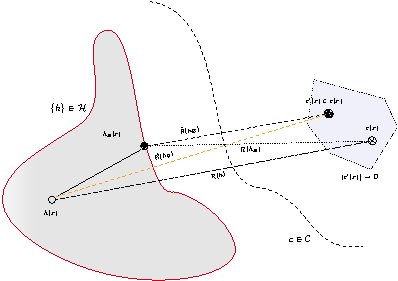
\includegraphics[width=0.6\textwidth]{pdf/figfig-crop.pdf}
    \caption{An illustration of statistical learning theory on the evaluation of the risks and errors, during learning process. $c'$ is presented in the `orbital' vicinity around $c$, with its distance of certain metric define how 'accurate' the reconstruction from distribution can be. Of the hypothesis set $\mathcal{H}$, there exists the Bayes hypothesis $h_{B}$ and an arbitrary `random' hypothesis $h$, and their respective measure.}
    \label{fig:genvsemp_fig}
\end{figure}

For the generalization problem's best model in a fixed $\mathcal{H}$, we have the notion of a \textbf{Bayes model}.\index{Bayes model}
\begin{definition}[Bayes risk]
    Given a distribution $\mathcal{D}$, the Bayes error $R^{*}$ is defined as the infimum of the errors achieved by measurable functions $h:\mathcal{X}\to \mathcal{Y}$: 
    \begin{equation}
        R^{*}=\underset{h\in \mathcal{H}}{\mathrm{inf}}R(h)
    \end{equation}
\end{definition}
\begin{definition}[Bayes model]
    A hypothesis $h$ with $R(h)=R^{*}$ is called a \textit{Bayes hypothesis} or Bayes classifier, and is taken by \begin{equation}
        \forall x\in \mathcal{X}, \quad h_{\mathrm{B}}=\argmax_{y\in\mathcal{Y}} \: \mathbb{E}[\ell(y,\mathcal{Y})|x] \equiv \underset{y\in \mathcal{Y}}{\mathrm{argmax}}\:\mathbb{P}[y\mid x]
    \end{equation}
    for the second equivalence on $h_{B}$ happens only in 0-1 regime loss.  
\end{definition}

The Bayes model is understood to be the minimal of $R(h)$. And, by our observations, $\hat{R}(h)\neq R(h)$ by a set of assumption on generalization access. In all, the dynamics depend on the commitment on $\Xi$ as the marginal error measure containing both itself. For now, we denote the risk as such, the goal of any system can be interpreted to minimize $\Xi$ in the learning setting. Thus, reframing the learning problem, we can give the following structural observation. 

\begin{theorem}[The general learning problem]
    We suppose the statistical, classical learning problem setting. Then, the learning problem of optimizing $(h,c)$ correlation, for $\mathcal{H},\mathcal{C}$ the hypothesis spaces and concepts space, on comparative (pseudo)measure $L\{\ell\}$ of which denotes a comparative objective functional, possibly composite, whose components include empirical and generalization terms, is the optimization for procedure $\mathcal{A}$, of which it produces the following model,
    \begin{equation}
        \argmin_{h\in\mathcal{H}}^{\epsilon\geq 0} L_{\ell}(h,c) \equiv \mathcal{A}\left(\mathcal{H},\Xi\right) = \mathcal{A}(\mathcal{H}, \hat{R}_{\mathcal{S}}(\cdot)+R(\cdot))
    \end{equation}
    where $\argmin_{h\in\mathcal{H}}^{\epsilon}$ is the $\epsilon$-minimum natural irreducible error without origin admission. If such model is efficient in $poly(\cdot)$ time, we say it is an \textbf{efficient algorithm} of the learning problem up to $\epsilon$-floor. Under such, $\mathcal{P}\equiv \mathcal{D}$. 
\end{theorem}

The notion would be generalized in the ongoing chapters, and the notation are being conveyed not particularly clear. However, as said, the main insight is this - the problem is between different $\epsilon$-tolerence class, of which affects the model and the algorithm process itself. Furthermore, as said, this learning problem setting presupposes \textbf{oracle enumerative access}, which is infinite sampling and distribution abstraction $\mathcal{D}$. Those are rather strong assumptions, and should be made explicit within the real, practical learning problem itself. For such, we would like to present another definition, with only a slight change of hand. 
\subsection{Instantiation of the learning problem - ordering}

When instantiate the setting of the learning problem, we are required to specify at least a sufficient domain validity of which the finite experiment can work on. Hence, while we can non-trivially but rather effortlessly define certain set of admissible working mechanisms, for example floating point precision abstraction, there are deliberately setting controlling methods on variations of the experimental setup that should be clarified. This can be said as for determining the \textbf{order of hyperparameter change order}, of which affects randomization patterns, reproducibility, and comparative class differences. We note this from now before moving on to later sections, as it is standard of the experimental preparation. 

Under the learning setting, there exists two types of \textbf{global hyperparameter}. We recall hyperparameter as a name assigned for non-learning mass of the model, which means they are conditioned on the setting of the learning setting itself. The two types are then accordingly, the \textbf{system hyperparameter}, and the \textbf{dynamic hyperparameter}, where the first one controls the space, for example, the space $\{\mathcal{S},\mathcal{H},\mathcal{C},[H_{1},\dots H_{k}]\}$ and so on for hyperparameters of the hypothesis, sample space, concept space, and another system parameters and specifications, which can includes the algorithm class $\mathbb{A}$. The second one, deliberately works on the instantiation of the hypothesis $h$, the concept space $c$ and its exposure, proxy $c'$, the parameters considering hypothetical $\mathcal{D}$, aggregated measures $\mathcal{P}$ on dataset-distribution, the controlling parameters of the design on $\mathcal{A}$-algorithm, and so on. 

The \textbf{specific hyperparameter}, contains hyperparameters that work upon the operation of specific algorithm or specific in operation construction. This includes step-size schedule, data feed, iterative constraints, where the global hyperparameter only specifies $N$ iteration, but we choose to only run $t=1$ time - which reduces it to analytical capable algorithm if one wants to justify the learning criteria. It also includes local outlier handling, procedural constraints, individual regularization patterns or the absence thereof, weighted decision template, kernel bandwidths, and so on, including dataset splitting in runtime, for example the 80-20 ratio between train and testing set. Those are often the region where it overlaps with the initial conditions specified by $[q_{1},\dots,q_{p}]$, since initial condition can be considered the specific hyperparameter operable of the algorithmic input, however in certain case, such can or cannot be the case. We note this tension of categorization in our attention. In all, the purpose of this separation is to showcase that there exists deliberate \textbf{clustered and nested layer} of construction, typically produced or controlled via parameterization into hyperparameters. Hence, specifically, to control experimental variations, the order is from global hyperparameter to downward to specific hyperparameters. This includes changing the $m$ sample size. This lies totally on the global hyperparameter, hence if one deliberately changes $m$ and also simultaneously change iterative patterns, but then change the high-level order of the global algorithm hyperparameters, it produces artefact of misalignment in hyperparameter control that cannot be taken into account. Hence, using such, in later section, we can also categorize the wide canonical family of double descent result into such order, where one then observe that epoch-wise double descent is of lower-order than the traditional double descent simply by hyperparameter ordering itself. 

\section{Optimal learning - PAC-learning}

The PAC-learning process (\cite{10.5555/2621980,10.5555/2371238,STL_Hajek_Maxim_2021}), or rather, \textit{Probably Approximately Correct} learning, connects three complexity measures - the sample space complexity, representation complexity, and optimization complexity, to the evaluation of the statistical learning process. It refers to the categorization of various learning procedure that satisfies the Probably Approximately Correct criteria in its name, as such being followed. The theory was proposed first by \cite{10.1145/1968.1972}, of whom then won the Turing Award, but his contribution stayed in the shadow in much of the end of the century, until the formal foundation of machine learning theory, of which then it becomes the stay ground on the standard discussion on the story of machine learner and algorithmic guarantees. As such, it is the de-facto foundation of statistical-based learning. The materials here based heavily on \cite{10.5555/2371238} and \cite{10.5555/200548}, aside from interpretations. 

For now, we assume no structure of $h$ and $c$. They can be functions, partial functions, relations, complex algorithms, or others. In a typically learning setting, we also have the argument of \textit{preliminary knowledge}, presented in literatures of the term \textit{inductive bias}. For example, if the concept class $\mathcal{C}$ is assumed, then we say the setting is \textbf{model-specific}. If there exists no hard assumption on $\mathcal{C}$, then the learning setting is said to be \textbf{model-free}. For clarification, we also use in the examples the 0-1 loss function, $\ell= \delta(h,c)$ for the Kronecker delta, such that the expected empirical risk is calculated as
\begin{equation}
    \hat{R}(h)=\frac{1}{n}\sum^n_{i=1}\delta_{h(\mathbf{x}_i)\ne y_i}, \quad \delta_{h(\mathbf{x}_i)\ne y_i}=\begin{cases}
        1,&\mbox{ $h(\mathbf{x}_i)\ne y_i$}\\
        0,&\mbox{ o.w.}
        \end{cases}
\end{equation} 
We can later on replace $\delta$ and the binary setting with others, albeit the complexity will increase on the formal derivation for others loss functions. One of the main reason why we often choose $0-1$ loss error in our analysis, comes from a variety of reasons. But, from what can be seen, it reduces the complexity of the problem, as well as raises the absoluteness of the loss measure. Indeed, naturally, from a soft point of view, the mean square loss measure is more natural of $\mathcal{L}_{2}$ norm on a representation space. As we have been saying, the loss function is chosen can influence the problem setting that one might expect the model to act on. $1-0$ measure effectively reduces the problem to the absolute \textit{binary classification problem}, where it is either correct or not. 

The \textit{learning algorithm} $\mathcal{A}$ can be interpreted to belong to a specific set of algorithm $\mathsf{A}$ such that it gives a sequence $\{ A_{i} \}$. If there exists such that $\lvert\{A_i\}\rvert=n$ for a fixed $n$, and can be explicitly defined and expressed, then the algorithm is \textit{deterministic}. Otherwise for arbitrary $m>1$ varying in magnitude, and with added uncertainty - that is, no sequence $\{A_i\}$ is the same, the algorithm is said to be \textit{probabilistic}, and by extension, a \textit{stochastic process}. We will give the definition of the stochastic process later on. Then, the algorithm is denoted by  $$\mathcal{A}=[h]\{ A_{1},\dots,A_{n} \}=\{ A_{i} \}_{i=1}^{n}$$
Under this line, we separate the classification of $c$ into two types: model-specific means that $c$ is deterministic - it is supposed to belong to certain class $\mathcal{C}$, or rather, its description can be contained into certain concept class (which ultimately is some priori). Model-free means that $c$ is not apparent to be able to separated to a concept class, which adds uncertainty, though all of them are still supposed to be at least a transformation $c:V\to U$ of arbitrary space $V,U$, by the setting of mathematical functional relationship. 
\begin{definition}[Model-specific learning]\index{model-specific learning}
    A learning scenario is called \textit{model-specific} learning if, for $R(h)$ being a measure-theoretic metric on the hypothesis $h$, we are given the dataset $D=\{ (\mathcal{X},\mathcal{Y}) \}$ with distribution $x\sim \mathcal{D}$, problem is to find a hypothesis $h\in\mathcal{H}$ that satisfies: \begin{equation}
        R(h) = \underset{x\sim \mathcal{D}}{\mathbb{P}} [h(x)\neq c(x)] = \underset{x\sim \mathcal{D}}{\mathbb{E}} [1_{h(x)\neq c(x)}]
    \end{equation}
\end{definition}

In the same way, we define the model-free learning, where the distribution is extended to $\mathcal{Y}$. This is to facilitate the uncertainty of the concept class. If the concept class $\mathcal{C}$ is deterministic, then there would be no ambiguity of the concept $c\in \mathcal{C}$ - we would only have to learn $\mathbb{P}(y\mid x)$, to predict or reconstruct accordingly. In such case, the only factor in consideration is the ground space $\mathcal{X}$, or rather, the relationship between $x$ and $y$ itself.\index{model-free learning} 

\begin{definition}[Model-free learning]
    A learning scenario is called \textit{model-free} learning if, for $R(h)$ being a measure-theoretic metric on the hypothesis $h$, we are given the dataset $D=\{ (\mathcal{X},\mathcal{Y}) \}$ with distribution $(x,y)\sim \mathcal{D}$. Problem is to find a hypothesis $h\in\mathcal{H}$ that satisfies \begin{equation}
        R(h) = \underset{(x,y)\sim D}{\mathbb{P}} [h(x)\neq y] = \underset{(x,y)\sim D}{\mathbb{E}} [1_{h(x)\neq y}]
    \end{equation}
\end{definition}
In both setting, we take the stance of absoluteness, using measure $\neq$, similar to a type of discrete decision process called \textit{classification}, for a finite class counts of the target class. This notion can be aggravated to be generalized to other classes, simply by replacing $h(x)\neq y$ by a valued-function, or by considering specific measure (for example, \textit{Bregman measure} for strictly convex functions). In the context of $n$-dimensional Euclidean space, and with the isomorphism $\mathbf{E}\simeq \mathbb{R}^{n}$ of suitable basis, the measure is simply the finite-accuracy Euclidean distance $d(h(x),c(x))$. 

Before analysing this problem in a PAC-like fashion, let us recall the setting in which we are operating upon. 
\begin{itemize}[topsep=0pt]
    \item The goal of the learning game is to learn an unknown target set, but the target set is not arbitrary. Instead, there is a known and rather strong constraint on the target set --- it is a rectangle in the plane whose sides are parallel to the axes. Under certain analysis, we can call this as having indeed a strong \textit{priori} to the concept $c\in \mathcal{C}$ possible. 
  
    \item Learning occurs in a probabilistic setting. Examples of the target rectangle are drawn randomly in the plane according to a fixed probability distribution which is unknown and unconstrained.
  
    \item The hypothesis of the learner is evaluated relative to the \textit{same} probabilistic setting in which the training takes place, and we allow hypotheses that are only approximations to the target. The tightest-fit strategy might not find the target rectangle exactly, but will find one with only a small probability of disagreement with the target. 
  
    \item We are interested in a solution that is efficient: not many examples are required to obtain small error with high confidence, and we can process those examples rapidly - that is, for time efficiency $t$. For it to be controllable, it is in our interest to know if we can run the learning process in polynomial time, that is, with $\mathrm{P}$-complexity class. 
  \end{itemize}

Ideally, we would want our model to be able to do the following: 
\begin{itemize}[itemsep=1pt,topsep=1pt]
    \item The number of calls to the concept $c$, or by extension, the oracle process $EX(c,\mathcal{D})$, is small, in the sense that it is bounded polynomially by some parameters. 
    \item The amount of computation performed is small. 
    \item The algorithm outputs a hypothesis $h$ such that $\Theta$ is small. Recall that $\Theta_{h} = (\hat{R}(h),R(h))$, but generally, the ideal goal would be to reduce to the infimum of $R(h)$. 
\end{itemize}

We are now ready to specify the definition of Probably Approximately Correct learning. For now, we designate this as a preliminary definition, because we will add more features into it. 

\begin{definition}[PAC Learning, Preliminary Definition]
    Let $\mathcal{C}$ be a concept class over $X$. We say that $\mathcal{C}$ is \textbf{PAC-learnable} if there exists an algorithm $\mathcal{L}$ that for every concept $c\in \mathcal{C}$, for every distribution $\mathcal{D}$ on $X$, and for all $0<\epsilon < 1/2$ and $0< \delta < 1/2$, if $\mathcal{L}$ is given access to $EX(c,\mathcal{D})$ for its output, and inputs $\epsilon, \delta$, then with probability at least $1-\delta$, outputs a hypothesis $h\in \mathcal{H}$ satisfying $R(h)\leq \epsilon$. This probability is taken over the random examples drawn by calls to $EX(c,\mathcal{D})$, and any internal randomization of $\mathcal{L}$. 

    If $\mathcal{L}$ further run in time polynomial in $1/\epsilon$ and $1/\delta$, we say that $\mathcal{C}$ is \textit{efficiently PAC learnable}. We will sometimes refer to the input $\epsilon$ as the \textbf{error parameter}, and the input $\delta$ as the \textbf{confidence parameter}.
\end{definition}

The hypothesis $h\in \mathcal{H}$ of the PAC-learning algorithm is thus approximately correct, with high probability, hence we got the name. Usually, $\mathcal{H}$ can not coincide with $\mathcal{C}$. However, a stronger form of the preliminary PAC-learning can set $h\in\mathcal{C}$, which guarantee the existence of a near-perfect hypothesis class. 

For the preliminary PAC learning model, there are two important problems with it, or rather, remarks on how it is constructed. 

First, the parameter pair $\epsilon, \delta$ control two types of failure to which a learning algorithm in the PAC model is inevitably susceptible. The error parameter $\epsilon$ is necessary since there may be only a negligible probability that a small random sample will distinguish between two competing hypotheses that differ on only one improbable point in the instance space. The confidence on only one improbable point in the instance (ground) space. The confidence parameter $\delta$ is necessary since the learning algorithm may occasionally be extremely unlucky, and draw a terribly "unrepresentative" sample of the target concept - for example, a sample consisting only of repeated draws of the same instances. The best we can hope for is that the probability of both types of failure can be made arbitrarily small at a modest cost. 

Second, we notice that we demand a PAC learning algorithm perform well with respect any distribution $\mathcal{D}$. This is a very strong requirement, which is moderated by the fact that we only evaluate the hypothesis of the learning algorithm with respect to the same distribution $\mathcal{D}$. Whether this is reduced or not, depends on the shape of which the distribution is induced via determination of distribution structure. 

\subsection{Representation size and PAC-configuration}

An important issue that has not been mentioned in our previous formation of PAC learning, is the fundamental distinction between a concept and its representation. 

Consider a class of concepts defined by the satisfying assignments of certain formulae. A concept from this class that satisfies such formulae, can be represented by a formula $f$, a truth table, or any given formulae that is tautologically equivalent formulae $f'$ to $f$. An example can be shown in high-dimensional Euclidean space $\mathbb{R}^n$, we may choose to represent a convex polytope (the hell is this?), we can specify the problem by either specifying its vertices, or specifying linear equations for its faces, and these two representation scheme, while being of the same problem, can differ in size. 

In each of these examples, we are fixing some representation scheme - that is, a precise method for encoding concepts \index{representation scheme}- and then examining the size of the encoding for various concepts. Other natural representation schemes that we are familiar it could be the vanilla neural network, or decision trees, though we cannot say exactly that the representation of neural network is indeed of the 'vanilla' representation. Taken example of the boolean formulae, for example, the boolean parity function $f(x_1,\dots,x_n)=x_1\oplus \dots\oplus x_n$ which can be computed by a circuit of $\land,\lor$ and $\lnot$ gates whose size is bounded by a fixed polynomial in $n$, but to represent this same function as a disjunctive normal form (DNF), requires size exponential in $n$. In these representation schemes, there is an obvious mapping from the representation (can be decision tree, or neural network) to the set or boolean function that is being represented. There is also a natural measure of the size of given representation in the scheme (for example, the number of weights, or neuron in a neural network). 

Since our PAC-learning algorithm for its model, follows the phenomenological interpretation, hence it is experimental data-only, it has absolutely no information about which, if any, of teh many possible representations is actually being used to represent the target concept in reality. However, it matters greatly which representation the algorithm chooses for its hypothesis, since the time to write this representation down is obviously a lower bound on the running time of the algorithm. At the end though, note that this is purely a computational concern at a glance, yet, further analysis into the problem might stem out certain consideration that previously unseen, for example, that fact that the representation scheme actually matters more in sense of a system analysis and its dynamic. 

Formally, a \textit{representation scheme} for a concept class $\mathcal{C}$ is defined as followed to capture this notion of representation size, and can be defined as below. 

\begin{definition}[Representation scheme]
    For a given concept class $\mathcal{C}$, a \textbf{representation scheme} for such concept class is a function $\bm{\mathcal{R}}: \Sigma^{*}\to \mathcal{C}$, where $\Sigma$ is the finite alphabet of symbols. We call any configuration $\sigma \in \Sigma^{*}$ such that $\bm{\mathcal{R}}(\sigma)=c$ a \textbf{representation} of $c$, under $\bm{\mathcal{R}}$. For any given $c$, the representation scheme might not be unique. \footnote{Perhaps representation scheme can be further realized by applying a Borel $\sigma$-algebra on top, and put on it a perspective measure to handle the notion of representation size. For example, in the traditional example of axis-aligned rectangle, one such representation scheme could be the real number schema $\bm{R}:(\Sigma \cup \mathbb{R})^{*}\to \mathcal{C}$, which then can utilize the extended notion of a Lebesgue measure over $\mathbb{R}$ and its spaces.}
\end{definition} 

To capture the notion of representation size, we assume that associated with $\bm{\mathcal{R}}$, there is a mapping size: $\Sigma^{*}\to N$ that assigns a natural number $size(h)$ to each representation $h\in \Sigma^{*}$. Note that we allow $size(\cdot)$ to be any such mapping results obtained under a particular definition for $size(\cdot)$ will be meaningful only if this definition is natural. In a more simple case, and arguably realistic setting, we can take $\Sigma=\{0,1\}$, thus, we have a binary encoding of concepts, and define $size(h)$ to be the length of $h$ in bits. Although we will use other definitions of size when binary representations are inconvenient, our definition of $size(\cdot)$ will always be within a polynomial factor of the binary string length definition.

So far, this definition is applicable only to representations, that is, to strings $h\in \Sigma^{*}$. We would like to extend this to $c\in \mathcal{C}$. Since the learning algorithm has access only to the input-output behaviour of $c$, in the worst case, it must assume that the simplest possible mechanism is generating this behaviour. Thus, we define $size(c)$ to be the infimum, that is: \index{representation size} \begin{equation*}
    size(c) = \min_{\bm{\mathcal{R}(\sigma)}=c}\{size(\sigma)\}
\end{equation*}
In other words, $size(c)$ is the size of the smallest representation of the concept $c$ in the underlying representation scheme $\bm{\mathcal{R}}$. While proceeding to the next section, a caution has to be made. Our notion of representative complexity lies fully within compressible string-expression system. That is, a model is reduced to its \textit{constructive description}, of which are records and protocols written on the computable tape. However, dynamics of the computation system lies within the changing state, thus there exists a blind gap in between this description of script length, and the actual instantiation. Rather, what would be present in a modern treatment, would be the initial-value-similar, \textit{static representational complexity} of a hypothesis class or concept class instead, with them being extension for the governed dynamical motions in dynamics, often ruled by algorithms or any specific active routines. 
\begin{definition}[Representation complexity]
    Given a concept $c\in\mathcal{C}$, the \textbf{representation complexity} of $c$ is defined to be the size of the smallest representation of the concept $c$ in the underlying representation scheme $\bm{\mathcal{R}}$, that is, 
    \begin{equation*}
    size(c) = \min_{\bm{\mathcal{R}(\sigma)}=c}\{size(\sigma)\}
\end{equation*}
for any string $\sigma$ of the representation scheme $\bm{\mathcal{R}}$ that still represents $c$.
\end{definition}
Under such definition, the more "complex" the concept $c$ is with the respective chosen representation scheme, the larger $size(c)$ is. This is also where the concept of the concept class $\mathcal{C}$ comes from - it comes from the \textit{representation class indiction} that we have in mind some fixed concept classes we study by their representation scheme. 

From this consideration of the representation size for the language in which the problem setting is expressed in, we gain the complete definition of PAC-learning for a fixed representation priori of the concept class. 

\begin{definition}[PAC-learning]
    A concept class $\mathcal{C}$ is said to be \textbf{PAC-learnable} if there exists an algorithm $\mathcal{A}$ and a polynomial function $poly(\cdot,\cdot,\cdot,\cdot)$ of 4-argument such that for any $\epsilon>0$, $\delta>0$, for all distribution $\mathcal{D}$ on $\mathcal{X}$ and for any target concept $c\in\mathcal{C}$, the following holds for any sample size $m\geq poly(1/\epsilon,1/\delta,n,size(c))$: $$\underset{S\sim \mathcal{D}^{m}}{\mathrm{Pr}}\left[ R(h(S))\leq \epsilon \right]\geq 1-\delta$$
    for a given error measure $R(h_{S})$. If $\mathcal{A}$ further runs in $poly(1/\epsilon,1/\delta,n,size(c))$, then $\mathcal{C}$ is said to be \textit{efficiently PAC-learnable}. When such algorithm exists, we call $\mathcal{A}$ a PAC-learning algorithm. 
\end{definition}

Finally, to compress the observations above. Current system operates within expression on binary systems, or rather computable substrate on $(0,1)^{n}$ string representation. Each string as such, encodes specific details, though not perfect, of the concept class within frame $Q$. Hence, any concept representation $c'$ in practice, now that we separate between $c$ and $c'$, can be considered exhibiting its structural details in different aspects from the dataset within such encoding. However, most of our construction in enumerative and numeral domains are \textit{of depth}, in the sense that the frame is rather complex and large to begin with. In most circumstances, the operating frame $Q_{f}$ for the financial frame, as such, encodes macroeconomic and certain simplification techniques, making it being sophisticated internally yet miniscule global of the unchartered descriptions. Natural extension to the question of general computing substrate than this, and whether or not dataset can be meaningfully and when constructed with full accuracy to the concept class, remains the open question, but generally efforts are fragmented and small (see inductive inference and extension for automata-based system and further on - we note that Turing machine is a rather poor choice in this problem, as there exists other representation of Turing machine that would not omit relevant details). Secondly, the algorithm constrain on polynomial factor $size(\cdot)$ is a polynomial equivalence condition. Different reasonable size measures as such are computationally equivalent, in the sense that \textit{generalizing in-between algorithm class} is possible, such that a polynomial-time algorithm under one size measure is a polynomial-time algorithm under any other, and the reverse on the algorithm class holds. This means that PAC learnability results, are invariant to the choice of size measure up to polynomial factors. This transfer across reasonable representation schemes, and thus condition a rather strong assumption about the description space, especially pre-dynamics. Most of the issues here, from identification of Layer II to Layer III, can be seen almost as artefact from Layer I to Layer II transition and choice. 

\subsection{Generalization bounds}

The theory based its goal around the target of \textbf{generalization learning problem}, hence, most of the bounds can be focus on achieving generalization target. Superficially, we assume the following is true of specific $h$ when trying to resolve the generalization problem. 
\begin{assumption}[Structural assumptions]
    We assume that $h\in\mathcal{H}$ is expressive enough on the hypothesis class, and algorithm $\mathcal{A}(h)$ is capable enough to extrapolate $h^{*}$ of the empirical best on the empirical space $\mathcal{S}$.
\end{assumption}
Under such assumption, to introduce the explicit objective of generalization bounds, we first need to introduce the categorization of the hypothesis based of one criterion: consistency. We say that an algorithm is a consistent learner for a concept class $C$ using hypothesis class $\mathcal{H}$, if for all $n$, for all $c\in C_n$ and for all $m$, given $\mathcal{S}$, as input, $x_i \in X_n$ outputs, then the algorithm $L$ outputs a hypothesis $h\in \mathcal{H}_n$ such that $h(x_i) = c(x_i) , i = 1,\dots,m$. Then $h$ is called the \textbf{consistent learner}. In other word, a consistent hypothesis is the hypothesis that is consistent with all the training data provided to it from the concept $c$. The following section contains the debate between consistent hypothesis (i.e., for example, admitting no error on training data, almost perfect - maybe even so), and inconsistent hypothesis, of which have general defects from the actual concept, or even different by a margin.  

Famous results contain two types of bound for classical PAC: the finite $\mathcal{H}$, and consistent hypothesis, and finite $\mathcal{H}$, but inconsistent. Infinite $\mathcal{H}$ assumes different stochasticity, and in consistent bound, generalization depends on the variances between empirical and generalization space, which is not covered in the theory, though in general setting the metric-induced distance can be small and controllable, which makes PAC applicable on said domain. For consistent case, we will consider the general sample complexity bound, or equivalently, a generalization bound for consistent hypothesis in the case where the cardinality $|\mathcal{H}|$ is finite. We will assume, as such, that the target concept $c$ is in $\mathcal{H}$. 

\begin{theorem}[Learning bound - finite $\mathcal{H}$, consistent case]
    \label{thm:consistent_case_thm_finite_H}
    Let $H$ be a finite set of functions mapping from $\mathcal{X}\to \mathcal{Y}$. Let $\mathcal{A}$ be an algorithm that for any target concept $c\in H$ and i.i.d. samples $S$ returns a consistent hypothesis $H_{S}$, such that $\hat{R}(h_{S}) = 0$. Then for any  $\epsilon,\delta>0$, the inequality $\mathrm{Pr}_{S\sim D^{m}}[R(h_{S})\leq \epsilon]\geq 1-\delta$ holds if $$m\geq \frac{1}{\epsilon}\left( \log{\lvert H \rvert }+\log{\frac{1}{\delta}} \right)$$
This sample complexity result admits the following equivalent statement as a generation bound: for any $\epsilon,\delta>0$, with probability at least $1-\delta$, 

\begin{equation}
    R(h_S) \leq \frac{1}{m} \left( \log{|\mathcal{H}|} + \log{\frac{1}{\delta}} \right)
\end{equation}
\end{theorem}

\begin{theorem}[Learning bound - finite $\mathcal{H}$, inconsistent case]
    \label{thm:inconsistent_case_thm_finite_H}
    Let $\mathcal{H}$ be a finite hypothesis set. Then, for any $\delta > 0$, with probability at least $1-\delta$, the following inequality holds: 
    \begin{equation}
        \forall h \in \mathcal{H}, \quad R(h) \leq \hat{R}_S (h) + \sqrt{\frac{\log{|\mathcal{H}|}+ \log{2/\delta}}{2m}}
    \end{equation}
\end{theorem}
The proofs are left in the Appendix section. In general, theorem~\ref{thm:consistent_case_thm_finite_H} shows that when the hypothesis set $\mathcal{H}$ is finite, a consistent algorithm $\mathcal{A}$ is a PAC-learning algorithm, since the sample complexity is dominated by a polynomial in $1/\epsilon$ and $1/\delta$. The generalization error of consistent hypothesis is upper bounded by a term that decrease w.r.t $m$. The decreases rate of $O(1/m)$ is guaranteed by this theorem. For the inconsistent theorem~\ref{thm:inconsistent_case_thm_finite_H}, it indicates that for a finite hypothesis set $\mathcal{H}$, then 
\begin{equation}
    R(h) \leq \hat{R}_S (h) + O \left( \sqrt{\frac{\log_{2}{|\mathcal{H}|}}{m}} \right)
\end{equation}
The term $\log{|\mathcal{H}|}$ can be interpreted as the number of bit needed to represent $\mathcal{H}$. A larger sample size $m$ guarantees better generalization, and the bound increases with $|\mathcal{H}|$, but only logarithmically. Note that the bound suggests seeking a trade-off between reducing the empirical error versus controlling the size of the hypothesis set: a larger hypothesis set is penalized by the second term but could help reduce the empirical error, that is the first term. But for a similar empirical error, it suggests using a smaller hypothesis set. This can be viewed as an instance of the so-called \textit{Occam's Razor}, of which can be said as: \textit{Plurality should not be posited without necessity}, or, the simplest explanation is best.

\subsection{Agnostic-general PAC-learning}

For the definition of PAC-learning in the above setting, for model-specific notion, there are some issues with it, more specifically, with the type of \textit{strong assumptions} that it holds. 
\begin{enumerate}[noitemsep,topsep=1pt]
    \item The \textit{representation size} and boundary only works for priori given of the concept class $\mathcal{C}$. In case that we cannot determine this, and there are a large potential for that to fail in capturing the minimal representation scope of the concept, the bound simply fails to a certain extent - given that our definition includes the polynomial bound of the concept class itself. 
    \item The assumption that the target concept $c$ belongs to $\mathcal{C}$ means that we are trying to fit a hypothesis to data, which are a priori known to have been generated by some member of the model class defined by $\mathcal{C}$. However, in general, we may not want to assume much about the data generation process, and instead would like to find the best fit to the data at hand using an element of some model class of our choice. 
    \item The assumption that the training features are labelled noiselessly rules out the possibility of noisy measurements or observations. 
    \item Even if the above assumptions were somehow true, we would not necessarily have a priori knowledge of the concept class $\mathcal{C}$, containing the priori knowledge of the concept class $\mathcal{C}$ containing the target concept or function. In that case, the best we could hope for is to pick our own model class and seek the best approximation to the unknown target concept among the elements of that class. 
\end{enumerate}

Agnostic case is considered the most general scenario of supervised learning, where the distribution $\mathcal{D}$ is defined over $\mathcal{X}\times \mathcal{Y}$, and the training data is a labelled sample $S$ drawn i.i.d. according to $\mathcal{D}$: 
$$S=\{ (x_{1},y_{1}),\dots,(x_{m},y_{m}) \}$$
The learning problem is to find a hypothesis $h\in \mathcal{H}$ with small generalization error
\begin{equation}
    R(h)=\underset{(x,y)\sim \mathcal{D}}{\mathbb{P}}[h(x)\neq y]=\underset{(x,y)\sim \mathcal{D}}{\mathbb{E}}[1_{h(x)\neq y}]
\end{equation}
This more general scenario is referred to as the stochastic scenario. Within this setting, the output target is a probabilistic function of the input. The stochastic scenario captures many real-world problems where the label of an input point is not unique\footnote{
    Considering two set $X$ and $Y$. A probabilistic function from $X$ to $Y$ assign to each $x\in X$ a relevant sub-distribution of elements of $Y$, rather than a single value $y\in Y$. Such a sub-distribution is a function $\delta: Y \to [0,1]$ such that $$\sum_{y\in Y}\delta(y)\leq 1$$In other words, a probabilistic function $X\to Y$ is a function $f: X\to (Y\to[0,1])$, interpreted as $f: X \times Y\to[0,1]$ such that for all $x\in X$, $$\sum_{y\in Y}f(x,y)\leq 1$$
}.
That said, the case of model-free is can be constructed in a simple manner, where we forgo any assumptions on the behaviours or structures of $\mathcal{C}$ and its associated $c$-model, and thus the observable pairs is simply $(x,y)\sim\mathcal{D}_{mf}$. Here, we denote $\mathcal{D}_{mf}$ to separate it from $\mathcal{D}$ of which is a singular $x$-distribution; however, we can also write $\mathcal{D}_{ms}$ and $\mathcal{D}_{mf}$ in certain specific cases. Per \cite{STL_Hajek_Maxim_2021}, the treatment of model-agnostic (no model $c$ assumption), targets the ingredient sets of, 
\begin{enumerate}[itemsep=1pt,topsep=1pt]
    \item Sets $\mathcal{X}, \mathcal{Y}$ and $\mathcal{U}$. Here, $\mathcal{U}$ is the correlated $h$-functional result, i.e. the hypothesis model, covering the case of \textbf{probabilistic models}. 
    \item A class $\mathcal{P}$ of probability distribution on $Z:=\mathcal{X}\times \mathcal{Y}$. Here, the distribution covers both. 
    \item A class $\mathcal{H}$ of functions $h:\mathcal{X}\to\mathcal{U}$. 
    \item A loss function as objective, $\ell: \mathcal{Y}\times \mathcal{U}\to[a,b]$, preferably $[0,1]$. Additional overhead measures are also required. 
\end{enumerate}

The \textit{agnostic PAC-learning} format is then modified by considering $\mathcal{Y}$ as also a random variability, and thus can be stated as followed.
\begin{definition}[Agnostic PAC-learning]
    A concept class $\mathcal{C}$ is said to be \textbf{PAC-learnable} if there exists an algorithm $\mathcal{A}$ and a polynomial function $poly(\cdot,\cdot,\cdot,\cdot)$ of 4-argument such that for any $\epsilon>0$, $\delta>0$, for all distribution $\mathcal{D}$  on $\mathcal{X}\times \mathcal{Y}$ and for any target concept $c\in\mathcal{C}$, the following holds for any sample size $m\geq poly(1/\epsilon,1/\delta,n)$:
    \begin{equation}
        \underset{S\sim \mathcal{D}^{m}}{\mathrm{Pr}}\left[ R(h(S))- \min_{h\in\mathcal{H}}R(h)\leq \epsilon \right]\geq 1-\delta
    \end{equation}
    If $\mathcal{A}$ further runs in $poly(1/\epsilon,1/\delta,n)$, then $\mathcal{C}$ is said to be \textit{efficiently agnostic PAC-learnable}. When such algorithm exists, we call $\mathcal{A}$ an agnostic PAC-learning algorithm.
\end{definition}

Under such lens, PAC-on-agnostic can be realized also using a more enumerative bound-on-definition instead: 
\begin{definition}[agnostic-PAC learning, \cite{STL_Hajek_Maxim_2021}]
    We say that a learning algorithm for a problem $(\mathcal{X},\mathcal{Y},\mathcal{U})$ and interpretations $(\mathcal{P},\mathcal{H},\ell)$ is PAC-learnable to accuracy $\epsilon > 0$, if, we have 
    \begin{equation}
        \lim_{n\to \infty}\sup_{P\in \mathcal{P}} P^{n} \left(Z^n : \hat{R}_{P}(h_{n})>\inf_{h\in\mathcal{H}} R_{P}(h)+\epsilon\right) = 0
    \end{equation}
    An algorithm that is PAC-learnable to accuracy $\epsilon$ for every $\epsilon >0$ is said to be a PAC-learning algorithm. A learning problem is said to be model-free learnable if there exists such algorithm, for every $A\in\mathcal{A}$ of such class to be \textbf{PAC}-learning algorithm class. 
\end{definition}

PAC-learning bound argues in the sense of \textit{computational complexities}, and \textit{space complexities}. Specifically, the term $poly(1/\epsilon,1/\delta,n,size(c))$ hopes to bound the required learning process to polynomial time, specified by 4 parameters. Here, $n$ is the \textit{input dimension}, $size(c)$ is the encoding complexity of the target concept, $\epsilon>0$ is the \textit{accuracy bound}, and $\delta$ is the confidence bound - the probability that $h$ fails.

\subsection{Empirical and structural algorithms}

Suppose that for a concept class $\mathcal{H}$, we can then partition it to $\mathcal{H}=\bigcup_{k\in \mathbb{N}} \mathcal{H}_{k}$ for finite $k$ hypotheses. Assume that they satisfy the uniform convergence (\cite{JMLR:v11:shalev-shwartz10a}), which means in the arbitrary path landscape, one can guarantee $\ell$-reduction, of $m$ samples on $\mathcal{S}$ to:

\begin{equation}
    \lim_{m\to \infty} \sup_{\mathcal{D}} \underset{S\sim\mathcal{D}^{m}}{\mathbb{E}} \left[ \sup_{h\in\mathcal{H}} [R(h) - R_{S}(h)] \right] = 0
\end{equation}

or, can also be expressed of equal to the following expression, for functions $\epsilon_{k}$ satisfies that for all $k$ and $\delta\in (0,1)$, $\lim_{m\to\infty}\epsilon_{k}=0$.

\begin{equation}
    \forall k \in \mathbb{N}, \quad \underset{S\sim \mathcal{D}^{m}}{\mathbb{P}} \left(\sup_{h\in \mathcal{H}_{k}} R(h) - \hat{R}_{S}(h)\leq \epsilon_{k}(m,\delta)\right) \geq 1- \delta
\end{equation}

Then such is said to be possible as a ruling dynamic when for a learning problem, the empirical risks of hypotheses in the hypothesis class converges to their population risk uniformly, with a distribution-independent rate. The result of this is that a problem then can be considered learnable with the ERM rule, for any given characterization. We state the following definition.\footnote{The reason why $r(\cdot)$ is not characterized in this preliminary section, is because of their uncertainty of effect. Hypothetically, $r(\cdot)$ is an additional structure (bias) of which apply a new gradient field in conjunction to the loss gradient field itself. This addition is uncertain of its content and analysis, since it depends on various stochastic dynamics of the model. We reserve from using regularization for now because of such reason.}

\begin{definition}
    A learning problem is learnable if there exist a learning rule $\mathcal{A}$ and a monotonically decreasing sequence $\epsilon_{cons}(m)$ such that $\epsilon_{cons}(m)\overset{m\to\infty}{\longrightarrow} 0$ and \begin{equation}
        \forall \mathcal{D} , \quad \underset{S\sim\mathcal{D}^{m}}{\mathbb{E}} \left[F(\mathcal{A}(S))-F^{*}\right] \leq \epsilon_{cons}(m),
    \end{equation}
    with $F^{*} = \inf_{h\in\mathcal{H}} R(h)$. A learning rule $\mathcal{A}$ for which this hold is denoted as a universally consistent learning rule. 
\end{definition}

There are certainly a fundamental class of rule or algorithm $\mathcal{A}$ to resolve this particular uniform convergence of classes. One of the major assumption or observation from the point of the hypothesis class, is that the hypothesis cannot know the generalization error. Thereby, one strategy is the \textit{empirical risk minimization} (ERM) method, minimizing only the empirical risk to the empirical best; then, certain measures to `generalize' this heuristically is apprehended on the hypothesis. 

\begin{definition}
    A rule $\mathcal{A}$ is an ERM (Empirical Risk Minimizer), denoted $\mathcal{A}_{ERM}$ if it minimizes the empirical risk $\hat{R}(h)=(1/m)\sum_{c\in\mathcal{C}}\ell(h,c)$, over the observational space $S$, 
    \begin{equation}
        \hat{R}_{S}(\mathcal{A}_{ERM}(S)) = \hat{R}_{S} (h_{S}) = \inf_{h\in\mathcal{H}} \hat{R}_{S}(h) 
    \end{equation}
    Hence, the ERM tries to obtain $\mathrm{ERM}(h') = \argmin_{h\in \mathcal{H}} \hat{R}(h)$. 
\end{definition}

The problem of overfitting still somewhat resides in the setting of the method. Hence, usually, we have an implicit term in addition, called the \textit{regularizer}, of which is as followed. 

\begin{definition}
    A rule $\mathcal{A}$ is an SRM (Structural Risk Minimizer), denoted $\mathcal{A}_{SRM}$ if it minimizes the empirical risk $\hat{R}(h)=(1/m)\sum_{c\in\mathcal{C}}\ell(h,c)$, over the observational space $S$, 
    \begin{equation}
        \hat{R}_{S}(\mathcal{A}_{SRM}(S)) = \hat{R}_{S} (h_{S}) + \lambda r(h)= \inf_{h\in\mathcal{H}} \hat{R}_{S}(h) + \lambda r(h)
    \end{equation}
    of the regularizing term $r(\cdot)$. Hence, the SRM tries to obtain $\mathrm{SRM}(h') = \argmin_{h\in \mathcal{H}} \hat{R}(h)+\lambda r(h)$, while taking into consideration a forcing term $r$, usually defined on the model complexity. 
\end{definition}

Hence, the SRM is inherently stronger than ERM. The regularizer $\lambda r(h)$, in specific case of convex loss landscape and reasonably well-behaved irregularities between domains, and of the structural regularization term $r_{s}(h)=\sum_{i,j}w_{ij}^{2}$ for weights of $ij$ index, then we have the following theorem. 

\begin{conjecture}[ERM-SRM growth]
    Consider the regulizer $\lambda r(h)$ for $h\in\mathcal{H}$. Assuming structural regularization $r_{\mathcal{S}}(h)=\sum_{i,j}w_{ij}^{2}$ for linear-layering of $ij$ index, for ERM and SRM optimizer classes, 
    \begin{equation}
    \begin{split}
        &\mathrm{ERM}\left(\inf_{h\in\mathcal{H}} \hat{R}_{S}(h), \ell\right)\\
        &\quad \quad \quad \approx o\left(\mathrm{SRM}\left(\inf_{h\in\mathcal{H}} \hat{R}_{S}(h) + \lambda r(h), [\ell ,\lambda r(h)]\right)\right)
    \end{split}
\end{equation}
\end{conjecture}

Where the little-$o$ notation is used for saying of the optimization strength per arbitrary time-similar notion of algorithmic evolution. The reason for this change is because of the restriction domain that $\mathrm{SRM}$ indicted on the model optimization landscape. Effectively, we introduce the structural bias $\lambda r(h)$ that forces the morph of the total loss landscape. In well-behaved case, this is usually effective to a point, however in realistic system and pathological cases, such can lead to the $c'$ approximation in $c$-space, just as we introduced in the reformulation of learning system. In this paper, we would like to presume the ERM method in question as the famous \textit{gradient descent}. We refer to \cite{achlioptas_stochastic_nodate,ruder_overview_2017} for general view of the algorithm, and \cite{zhang_gradient_2019} for a source on particularly gradient descent algorithm on deep learning models. 

One particularly troublesome and should take serious consideration into interpreting it, is the fact of the insufficiency on ERM. The following proposition is rather questionable. 
\begin{proposition}
    For any sample $S$, the following inequality holds for the hypothesis returned by ERM: 
    \begin{equation}
        \mathbb{P}\Big[R(h_{S}')- \inf_{h\in \mathcal{H}}R(h) > \epsilon\Big] \leq \mathbb{P}\Big[ \sup_{h\in \mathcal{H}} \lvert R(h)- \hat{R}_{S}(h) \rvert > \frac{\epsilon}{2} \Big]
    \end{equation}
\end{proposition}
We will prove this proposition in later section. For now, this proposition bounds the error of ERM, with respect to the probability of the generalization distance $\lvert R(h)- \hat{R}_{S}(h)\rvert$ between the two errors. As we might have suspected, the performance of ERM is typically very poor. This is because the algorithm disregards the complexity of the hypothesis set $\mathcal{H}$: in practice, either it is not complex enough, in which case the error can be large, or $\mathcal{H}$ is so rich, that the complexity makes the model shoot out of the complexity range. Additionally, in many cases, determining the ERM solution is computationally intractable. 

\subsection{The PAC-ERM notion}

Without restricting ourselves to specific ERM construction, we can still apply PAC on the set of ERM algorithms in its generality of itself. Within such understanding, the empirical risk minimization strategy is often motivated by the hope that \textit{$R$(h) and $\hat{R}(h)$ are not too far-distant apart}. Particularly, it also implicitly agree with statements conjectured with law of large number, for $n\to\infty$, $|R(h)-\hat{R}(h)|\approx \epsilon$ of irreducible noise. To what extent is this true, we have to take certain boundary on which might have been previously shown. We refer to authoritative introductory texts like \cite{Alquier_2024}, for both PAC-ERM and later sections on PAC-Bayes variation. 

\begin{proposition}[\cite{Alquier_2024}]\label{prop:PAC_ERM_1}
    For any $h\in\mathcal{H}$, for any $\delta\in(0,1)$, 
    \begin{equation}
        \mathbb{P}_{S}\left( R(h) > \hat{R}(h)+ C\sqrt{\frac{\log{(1/\delta)}}{2n}}\right)\leq \delta
    \end{equation}
\end{proposition}
\begin{proof}
    Applying Hoeffding's inequality onto $U=\mathbb{E}[\ell_{i}(h)]-\ell_{i}(h)$, 
    \begin{equation}
        \mathbb{E}_{S}\left[\exp{tn[R(h)-\hat{R}(h)]}\right] \leq \exp{[(nt^2C^2)/8]}
    \end{equation}
    For any $s>0$, we have by Markov's inequality, 
    \begin{equation}
        \begin{split}
            \mathbb{P}_{S}(R(h)-\hat{R}(h)>s) 
            & = \mathbb{P}_{S} \left(\exp{nt[R(h)-R]}> \exp{(nts)}\right)\\
            & \leq \frac{1}{\exp{(nts)}} \mathbb{E}_{S}\left[e^{nt[R(h)-\hat{R}(h)]}\right]\\
            & \leq \exp{\left(\frac{nt^2C^2}{8}-nts\right)}
            \end{split}
    \end{equation}
    We can make this bound as tight as possible, by optimizing the choice of $t$. For $t=4s/C^{2}$, we have 
    \begin{equation}
        \mathbb{P}(R(h)-\hat{R}(h)>s) \leq \exp{\left(\frac{-2ns^2}{C^2}\right)}
    \end{equation}
    This means that, for a given $h$, the empirical risk $\hat{R}(h)$ cannot be much smaller than the risk $R(h)$. The order of this "much smaller" can be better understood by introducing $\delta=\exp{(-2ns^2/C^2)}$, of which substituting $\delta$ to $s$ yields the required proposition. 
\end{proof}

Proposition~\ref{prop:PAC_ERM_1} bounds the asymptotic term such that $R(h)$ will exceed $\hat{R}(h)$ by certain margin, at worst $1/\sqrt{n}$. However, this is not enough to justify the use of ERM (which indeed use the near-space approximation from empirical to general risk), since the proof only applies for $h$ that was fixed above in terms of complexity. For those that is implicit of the data itself, we cannot apply them\footnote{This means models such ass \textit{support vector machine} (SVM) or \textit{Gaussian process regression} of which the empirical optimization function and the hypothesis itself, relies on the number of data points available.}. The usual approach though, is to use the inequality 
\begin{equation}
    R(h_{ERM}) - \hat{R}(h_{ERM}) \leq \sup_{h\in\mathcal{H}} \left[R(h)-\hat{R}(h)\right]
\end{equation}
and to prove a version of Proposition~\ref{prop:PAC_ERM_1} that would hold uniformly on $\mathcal{H}$. 
\begin{theorem}
    Assume that $\mathrm{card}(\mathcal{H})=M<+\infty$, for any $\delta\in(0,1)$, 
    \begin{equation}
        \mathbb{P}_{S}\left( R(h_{ERM}) \leq \inf_{h\in\mathcal{H}} \hat{R}(h) + C\sqrt{\frac{\log{(M/\delta)}}{2n}} \right) \geq 1 - \delta
    \end{equation}
\end{theorem}
\begin{proof}
    We upper bound the supremum in the inequality by 
    \begin{equation}
        \begin{split}
            \sP_{S} \left(\sup_{h\in\mathcal{H}}[R(h)-\hat{R}(h)>s]\right)
            & = \sP_{S} \left(\bigcup_{h\in\mathcal{H}} \left\{ [R(h)-\hat{R}(h)]>s \right\} \right)\\
            & \leq \sum_{h\in\mathcal{H}} \mathbb{P}_{S}(R(h)-\hat{R}(h)>s)\\
            & \leq M\exp{\left(\frac{-2ns^2}{C^2}\right)}
        \end{split}
    \end{equation}
    This time, put $\delta = M\exp{(-2ns^2/C^2)}$ we gain 
\begin{equation}
     \mathbb{P}_{S}\left( \sup_{h\in\mathcal{H}}[R(h)-\hat{R}(h)] \leq  C\sqrt{\frac{\log{(M/\delta)}}{2n}} \right) \leq \delta
\end{equation}
Thus it satisfies 
\begin{equation}
     \mathbb{P}_{S}\left( \sup_{h\in\mathcal{H}}[R(h)-\hat{R}(h)] \leq  C\sqrt{\frac{\log{(M/\delta)}}{2n}} \right) \geq 1-\delta
\end{equation}
Using the inequality
\begin{equation}
    \mathbb{P}_{S}\left( R(h_{ERM}) \leq \hat{R}(h_{ERM})  C\sqrt{\frac{\log{(M/\delta)}}{2n}} \right) \geq 1-\delta    
\end{equation}
As $\mathcal{H}$ is finite, $\hat{R}(h_{ERM})=\inf_{h\in\mathcal{H}}\hat{R}(h)$.
\end{proof}
This bound coincides for the \textit{Probably Approximately Correct} PAC-bounds, specifically for algorithm of ERM principle, since it approximates $R(h_{ERM})$ within $C\sqrt{\log{(M/\delta)}/2n}$ with probability $1-\delta$, and once again, under very strong arguments. Certain version of this theorem's result can be derived to `predict' double descent, but not giving its the diagnostic view. 
\subsection{Noise, \cite{10.5555/2371238}}

Using the notion of the Bayes classifier and Bayes error, one can define the \textit{noise} \index{noise} of a given learning setting under PAC-learning consideration, as followed. 
\begin{definition}[Noise]
    Given a distribution $\mathcal{D}$ over $\mathcal{X}\times \mathcal{Y}$, the \textit{noise} at point $x\in \mathcal{X}$ is defined by \begin{equation*}
        noise(x) = \min_{x\in \mathcal{X}} \{\mathbb{P}[1\mid x], \mathbb{P}[0\mid x]\}
    \end{equation*}
    The average noise or the noise associated to $\mathcal{D}$ is then the minimum possible error aside from intrinsic model error, and is calculated by $\mathbb{E}[noise(x)]$
\end{definition}
Thus, the average noise is precisely the Bayes error, that is, $noise = \mathbb{E}[noise(x)]=R^{*}$. The noise is a characteristic of the learning task indicative of its level of difficulty. A point $x\in \mathcal{X}$, for which noise is close to $1/2$, is sometimes referred to as \textit{noisy} and is of course a challenge for accurate prediction. Such is understandable, and is often enough, however, we note that structurally, it is missing particular components or decomposition components that would eventually make up the builks of its claims. 

\section{Simplistic learning - Occam's Razor}

The PAC model that we introduced defined learning directly in terms of the predictive power of the hypothesis output by the learning algorithm. That is, given a hypothesis $h\in \mathcal{H}$ and the learning algorithm $\mathcal{L}$, the learning involves switching this dynamic of the predictive power of the hypothesis, over certain setting and problem. We can, as it is possible to apply this measure, to a learning algorithm because we made the assumption that the instances are drawn, from a probabilistic perspective, from a fixed distribution $\mathcal{D}$ then measured the predictive power with respect to the same distribution. 

Our new notion, dubbed as \textit{Occam learning} (our source is mainly taken from the exposition of \cite{10.5555/200548}), would let us consider a different definition of learning that makes no assumptions about how the instances in a labelled sample are chosen, though we will assume that the labels are generated by a target concept chosen from a known class. Instead of measuring the predictive power of a hypothesis, the new definition judges the hypothesis by how succinctly it explains the observed data (or a labelled example). The crucial difference between PAC learning and Occam learning, is then that in PAC learning, the random sample drawn by the learning algorithm is intended only as an aid for reaching an accurate model of some external process, while in the new definition, we are concerned only with the fixed sample before us, and not any external process. By that, we simply reduce it to somewhat similar of the statistical estimation problem setting, though not exactly the same. 

This also contains the substance of which we often call the \textit{Occam's razor}, telling that overly complex scientific theories should be subjected to a simplifying knife. If we equate "simplicity" with representational succinctness, then another way to interpret Occam's razor would be to say learning is the act of finding a pattern in the observed data that facilitates a compact representation or compression of this data. In our simple concept learning setting, succinctness is measured by the size of the representation of the hypothesis concept. Equivalently, we can measure succinctness by the cardinality of the hypothesis class used by the algorithm, for if this class is small then a typical hypothesis from the class can be represented by a short binary string, and if this class is large then a typical hypothesis must be represented by a long string. Thus, an algorithm is an \textit{Occam algorithm} if it finds a short hypothesis consistent with the observed data. 

Additionally so, it would be plenty interesting to see that Occam's razor somehow falls into the range of what would be expected of the \textit{bias-variance tradeoff}. This perhaps, will prompt us to push further into the inquiry of double descent, which empirically, breaks the principle of the Lord William Occam. 

\subsection{Occam Learning and Succinctness}

Let $X= \cup_{n\geq 1} X_n$ be the instance space, let $\mathcal{C}=\cup_{n\geq 1}\mathcal{C}_{n}$ be the target concept class, and let $\mathcal{H}= \cup_{n\geq 1}\mathcal{H}_{n}$ be the class of hypothesis representation. The notation is preferably clarified: $X_{n}$ is under the binary representation typically concerned $\{0,1\}^{n}$, or a boolean string of length $n$. Hence, $\mathcal{H}_{n}$ and $\mathcal{C}_{n}$ are subsequently concept and hypothesis class specified for such string space. In this part, we will assume, unless explicitly stated otherwise, that the hypothesis representation scheme of $\mathcal{H}$ uses a binary alphabet, and we define $size(h)$ to be the length of the bit string $h$. Also, recall that for a concept $c\in \mathcal{C}$, $size(c)$ denotes the size of the smallest representation of $c$ in $\mathcal{H}$. Let $c\in \mathcal{C}_{n}$ denote the target concept. A labelled sample $S$ of cardinality $m$ is a set of pairs: \footnote{This section is taken, and studied, from a pretty old book. It would be then observed that a lot of the concept, including the representation, is taken in a rather computer science fashion such as for the hypothesis $\mathcal{H}$ to be binary representation.}
\begin{equation*}
    S = \{(x_1, c(x_1)),\dots,(x_m, c(x_m))\}
\end{equation*}
An \textbf{Occam algorithm} $L$ takes as input a labelled sample $S$, and outputs a short hypothesis $h$, "relatively so", that is consistent with $S$. By consistent, we mean as one definition above, $h(x_{i})= c(x_{i})$ for each $i$, and for short we mean that $size(h)$ is a sufficiently slowly growing function of $n$, $size(c)$ and $m$. This is formalised in the following definition. 

\begin{definition}[Occam algorithm]
    Let $\alpha \geq 0$ and $0\leq \beta < 1$ be constant. $L$ is an $(\alpha, \beta)$-\textbf{Occam algorithm} for $\mathcal{C}$ using $\mathcal{H}$ if on input a sample $S$ of cardinality $m$ labelled according to $c\in \mathcal{C}_{n}$, $L$ outputs a hypothesis $h\in \mathcal{H}$ such that: 
    \begin{itemize}[itemsep=1pt,topsep=1pt]
        \item $h$ is consistent with $S$, or $h(x_{i})=c(x_i)$ for all $x_{i}\in S_{x}$. 
        \item $size(h)\leq (n\cdot size(c))^{\alpha}m^{\beta}$
    \end{itemize}
    We say that $L$ is an \textbf{efficient} $(\alpha,\beta)$-Occam algorithm if its running time is bounded by a polynomial in $n,m$ and $size(c)$.  
\end{definition}

The growth complexity $\mathcal{O}(n\cdot size(c))^{\alpha} m^{\beta}$ is somewhat difficult to scale down. However, we can somewhat try to prove if it is convergence or not. 

\begin{theorem}
    Fix $n$. Then $\mathcal{O}(n\cdot size(c))^{\alpha} m^{\beta}$ is convergence or divergence depends on the ratio of $\alpha$ and $\beta$. 
\end{theorem}
\begin{proof}
    Fixed $n$, then we have the class $\mathcal{C}_{n}$ to be finitely restricted of $n$ representation class. Then, $size(c)$ for $c\in \mathcal{C}$ is also constant. We then reduce the first complexity measure to be $\mathcal{O}(\lambda^{\alpha} m^{\beta})$. Since $0\geq\beta < 1$, it follows that as $\beta$ increase, $size(h)$ monotonically decrease. This is also the case for $\alpha$ in range $[0,1)$. Hence, it converges to at least $n$, and diverges accordingly for arbitrary $\alpha>1$, though the trend will not as strong if $m> n$, or $m\gg n$. 
\end{proof}

Now, in what sense can we say that the output $h$ of an Occam algorithm succinct? First, let us assume that $m\gg n$, so that the above bound can be effectively simplified to $size(h)< m^{\beta}$, for some $\beta < 1$. Since the hypothesis $h$ is consistent with the sample $S$, $H$ allows us to reconstruct the $m$ labels $c(x_1) = h(x_1),\dots,c(x_m)=h(x_m)$, and is given only the unlabelled sequence of instance $x_{1},\dots,x_{m}$. Thus the $m$ bits $c(x_1),\dots,c(x_m)$ have been effectively \textit{compressed} into a much shorter string $h$ of length at most $m^{\beta}$. Note that the requirement $\beta<1$ is quite weak, since a consistent hypothesis of length $O(mn)$ can always be achieved by simply storing the sample $S$ in a table (at a cost of $n+1$ bits per labelled example) and giving an arbitrary answer for instances that are not in the table. We would be certainly not expecting such a hypothesis to have any predictive power. 

By sheer observation of the definition we have been constructing, the $(1,0)$-Occam algorithm is the largest deviation, with the bound $size(h)\leq n \cdot size(c)$. This means it can at most, have the representation size equal to \textit{all} representation partition of $c\in \mathcal{C}$. It is also good to note the misconception, or rather the misinterpretation: $size(c)$ is different from $n$, even though they are particularly the same from first glance. It is because $n$ is actually the representation size of the instance string, and not the concept representation string, which utilizes another alphabet entirely. Though, suppose they are of the same alphabet, then $X= \{\Sigma\}_{n}$, then again, there exists a number $q$ such that $q \geq n$. In the case where $q=n$, it is most likely that the representation is constrained of the linear transformation order, of which does not change the string length. 

Let us observe that even in the case $m\ll n$, the shortest consistent hypothesis in $\mathcal{H}$ may in fact be the target concept, and so we must allow $size(h)$ to depend at least linearly on $size(c)$. We will see cases where this makes it easier to efficiently find a consistent hypothesis --- by contrast, computing the shortest hypothesis consistent with the data is often a computationally hard problem. 

\begin{theorem}[Occam's Razor]\label{thm:Occam1}
    Let $L$ be an efficient $(\alpha,\beta)$-Occam algorithm for $\mathcal{C}$ using $\mathcal{H}$. Let $\mathcal{D}$ be the target distribution over the instance space $X$, let $c\in \mathcal{C}_{n}$ be the target concept, and $0< \epsilon, \delta \leq 1$. Then there is a constant $a>0$ such that if $L$ is given as input a random sample $S$ of $m$ examples drawn from $EX(c,\mathcal{D})$, where $m$ satisfies: 
    \begin{equation}
        m \geq a \left( \frac{1}{\epsilon} \log{\frac{1}{\delta}} + \left(\frac{(n\cdot \mathrm{size}(c)^{\alpha})}{\epsilon}\right)^{1/1-\beta} \right)
    \end{equation}
    then with probability at least $1-\delta$ the output $h$ of $L$ satisfies $error(h)\leq \epsilon$. Moreover, $L$ runs in time polynomial in $n$, $size(c)$, $1/\epsilon$ and $1/\delta$.  
\end{theorem}
Notice that as $\beta$ tends to 1, the exponent in the bound for $m$ tends to infinity. This corresponds with the assumption of intuition that the length of the hypothesis approaches that of the data itself, then the predictive power of the hypothesis is diminishing. 

To apply this theorem into variational setting, we turn to the arguably more general definition, measuring representational succinctness by the cardinality of the hypothesis class rather than the representationally supposed bit length $size(h)$. Then, theorem~\ref{thm:Occam1} will be the special case of such theorem. To make this precise, let $\mathcal{H}_{n}= \cup_{m\geq 1}\mathcal{H}_{n,m}$.

\begin{theorem}[Occam's Razor, Cardinality Version]\label{thm:Occam2}
    Let $\mathcal{C}$ be a concept class and $\mathcal{H}$ a representation space. Let $L$ be an algorithm such that for any $n$ and any $c\in \mathcal{C}_{n}$, if $L$ is given as input a sample $S$ of $m$ labelled examples of $c$, then $L$ runs in time polynomial in $n$, $m$, and $size(c)$, and output an $h\in \mathcal{H}_{n,m}$ that is consistent with $S$. Then there is a constant $b>0$ such that for any $n$, any distribution $\mathcal{D}$ over $X_{n}$, and any target concept $c\in \mathcal{C}_{n}$, if $L$ is given as input a random sample from $EX(c,\mathcal{D})$ of $m$ examples, where $|\mathcal{H}_{n,m}|$ satisfies: 
    \begin{equation}
        \log{|\mathcal{H}_{n,m}|} \leq b \epsilon m - \log{\frac{1}{\delta}}
    \end{equation} 
    or equivalently, where $m$ satisfies $m\geq (1/b\epsilon)(\log{|\mathcal{H}_{n,m|}}+ \log{(1/\delta)})$ then $L$ is guaranteed to find a hypothesis $h\in \mathcal{H}_{n}$ that with probability at least $1-\delta$ obeys $error(h)\leq \epsilon$. 
\end{theorem}
We do not mention, or necessarily claim that $L$ is an efficient PAC learning algorithm. In order for the theorem to apply, we must pick $m$ large enough so that $b\epsilon m$ dominates $\log{|\mathcal{H}_{n,m}|}$. 

\begin{proof}[Proof of Theorem~\ref{thm:Occam2}]
    We first give a proof of theorem~\ref{thm:Occam1}, by proving the more general form in theorem~\ref{thm:Occam2}, of which then is considered a special case to prove. Firstly, we say that a hypothesis $h\in \mathcal{H}_{n,m}$ is \textit{bad} if $error(h)>\epsilon$, where the error is of course measured with respect to the target concept $c$ and the target distribution $\mathcal{D}$. Then, by the independence of the random examples, the probability that a fixed bad hypothesis $h$ is consistent with a randomly drawn sample of $m$ examples from $EX(c,\mathcal{D})$ is at most $(1-\epsilon)^{m}$. Using the union bound, this implies that if $\mathcal{H}'\subseteq \mathcal{H}_{n,m}$ is the set of all bad hypotheses in $\mathcal{H}_{n,m}$, then the probability that some hypothesis in $\mathcal{H}'$ is consistent with a random sample of size $m$ is at most $|\mathcal{H}|(1-\epsilon)^{m}$. We want this to be at most $\delta$, since $|\mathcal{H}'|\leq |\mathcal{H}_{n,m}|$ we get a stronger condition if we solve for $|\mathcal{H}_{n,m}|(1-\epsilon)^{m}\leq \delta$. From this, we obtain 
    \begin{equation}
        \log{|\mathcal{H}_{n,m}|} \leq m \log{(1/1-\epsilon)} - \log{(1/\delta)}
    \end{equation}
    Using the fact that $\log{(1/1-\epsilon)}=\Theta(\epsilon)$, we get the statement of the theorem. 
\end{proof}

\begin{proof}[Proof of Theorem~\ref{thm:Occam1}]
    Let $\mathcal{H}_{n,m}$be the set of all possible hypothesis representation that the $(\alpha,\beta)$-Occam algorithm $L$ might output when given as input a labelled sample $S$ of cardinality $m$. 

    Since $L$ is an $(\alpha,\beta)$-Occam algorithm, every such hypothesis has bit length at most $(n\cdot size(c))^{\alpha}m^{\beta}$, thus implying that $|\mathcal{H}_{n,m}|\leq 2^{(n\cdot size(c))^{\alpha}m^{\beta}}$. By Theorem~\ref{thm:Occam2}, the output of $L$ has error at most $\epsilon$ with confidence at least $1-\delta$, provided 
    \begin{equation}
        \log{|\mathcal{H}_{n,m}|} \leq b\epsilon m - log{\frac{1}{\delta}}
    \end{equation}
    Transposing, we want $m$ such that 
    \begin{equation}
        m\geq \frac{1}{b\epsilon} \log{|\mathcal{H}_{n,m}|} + \frac{1}{b\epsilon}\log{\frac{1}{\delta}}
    \end{equation}
    The above condition can be satisfied by picking $m$ such that both \begin{equation}
        m\geq \left(\frac{2}{b\epsilon}\right) \log{|\mathcal{H}_{n,m}|} , \quad m \geq \left(\frac{2}{b\epsilon}\right) \log{\frac{1}{\delta}}
    \end{equation}
    will effectively hold. Choosing $a=2/b$ yields the statement in the theorem. \footnote{Why is the pairing of $(a,b)$ value is as such, we are not so sure.}
\end{proof}



\section{Discrete space empiricism - Rademacher complexity}

The jump toward discrete space is natural, as information are often discrete on infinite and continuous phase space (i.e. the domain, for example, $\mathbb{R}$-values). The hypothesis sets typically used in machine learning are infinite, even in toy model, as the rectangular learning problem itself can be expressed by infinitely many rectangles. But the sample complexity bounds are uninformative when dealing with infinite hypothesis sets - for arbitrary construction of $\mathcal{H}$. One could ask whether efficient learning from a finite sample is even possible when the hypothesis set $\mathcal{H}$ is infinite. The basic goal with the Rademacher complexity is this exact question, for the first complexity treatment. The general idea for doing so consists of reducing the infinite case to the analysis of finite sets of hypotheses, and then proceed as previous sections. Authoritative sources provided mainly the insight and theories in this section, as of \cite{10.5555/2371238} and \cite{bartlett2002rademacher}. 

\subsection{Rademacher descriptions}
We will continue to use $\mathcal{H}$ to denote a hypothesis set as in the previous chapters. Many of the result of this section are general and hold for arbitrary loss function, or $L: \mathcal{Y}\times \mathcal{Y}\to \mathbb{R}$. In what follows, $\mathcal{G}$ will generally be interpreted as the \textit{family of loss functions associated to $\mathcal{H}$}, mapping from $\mathcal{Z}=\mathcal{X}\times\mathcal{Y}$ to $\mathbb{R}$. That is, \begin{equation*}
    \mathcal{G} = \{g: (x,y)\mapsto L(h(x),y): h\in \mathcal{H}\}
\end{equation*}
However, the definitions are given in the general case of a family of arbitrary functions $\mathcal{G}$, mapping from an arbitrary input space $\mathbb{Z}$ to $\mathbb{R}$. Thus, we can say that we endowed upon the landscape a measure set $\mathcal{G}$ of all singular mapping. 

The \textbf{Rademacher complexity} captures the richness of a family of functions by measuring the degree to which a hypothesis set can fit random noise. This is perhaps one of the very \textit{empirical complexity notion} that would be seen, as for the random noise idea, that is. \index{ERC}

Let $G$ be a family of functions mapping from $Z\to [a,b]$, $S=(z_1,\dots, z_m)$ a fixed sample of size $m$ with elements in $Z$. Then, the \textbf{empirical Rademacher complexity} of $G$ with respect to the sample $S$ is defined as:
\begin{equation*}
    \hat{\mathfrak{R}}_S (\mathcal{G}) = \mathbb{E} \left[ \sup_{g\in G} \frac{1}{m} \sum^{m}_{i=1} \sigma_i g(z_i) \right]
\end{equation*}
where $\bm{\sigma}=\{\sigma_1,\dots,\sigma_m\}^{\top}$ with $\sigma_i$s independent uniform random variables taking values in $\{-1,+1\}$. The random variable $\sigma_i$ are called \textbf{Rademacher variables}.\index{Rademacher variables} 

The empirical Rademacher complexity can be rewritten as:
$$\hat{\mathfrak{R}}_S (\mathcal{G}) = \underset{\mathbf{\sigma}}{\mathbb{E}} \left[\sup_{g \in G} \frac{\bm{\sigma}\cdot \mathbf{g}_S}{m}\right]$$
for $\mathbf{g}_S$ denoting the vector of values taken by $g$ over the sample $S$: $\mathbf{g}_{S} = (g(z_1),\dots,g(z_{m}))^{\top}$. The inner product measures the correlation of $\mathbf{g}_{S}$ with the vector of random noise $\bm{\sigma}$. The supremum $\sup_{g\in \mathcal{G}} (\bm{\sigma}\cdot \mathbf{g}_{S}/m)$ is a measure of how well the function class $\mathcal{G}$ correlates with $\bm{\sigma}$ over the sample $S$. Thus, the empirical Rademacher complexity measures on average how well the function class correlates with random noise on the dataset. What will the random noise be like? Well, not much. For a fixed sample size, it captures how \textbf{random} the loss function distribution is. A random noise system is inherently chaotic by default, even if we restrict its value in $\{-1,+1\}$ \footnote{Actually, this is indeed a problem. What will happen if the value is totally synchronous for a specific configuration that is, though statistically impossible, yet is the solution to the finite space?}. Hence, if the model is good enough on certain dataset, that the noisy, useless data configuration performs "somewhat pretty well", then from that, we can know the complexity of the model by its flexibility in such noisy fitting. That is, in the topic of fitting, at least. So the richer or more complex families $\mathcal{G}$ can generate more vectors $\mathbf{g}_{S}$ and thus better correlate with random noise on average. 

We come to the definition of \textit{the} Rademacher complexity. \index{Rademacher complexity}
\begin{definition}[Rademacher complexity]
    Let $\mathcal{D}$ denote the distribution according to which samples are drawn. For any integer $m\geq 1$, the \textbf{Rademacher complexity} of $\mathcal{G}$ is the expectation of the empirical Rademacher complexity over all samples of size $m$ drawn according to $\mathcal{D}$. 
    \begin{equation}
        \mathfrak{R}_{m} (\mathcal{G}) = \underset{S\sim \mathcal{D}^{m}}{\mathbb{E}} [\hat{\mathfrak{R}}_{S}(\mathcal{G})]
    \end{equation}
\end{definition}

We are now ready to present our first generalization bound based on Rademacher complexity. 

\begin{theorem}
    Let $\mathcal{G}$ be a family of functions mapping from $\mathcal{Z}$ to $[0,1]$. Then, for any $\delta > 0$, with probability at least $1-\delta$ over the draw of an i.i.d. sample $S$ of size $m$, each of the following holds for all $g\in \mathcal{G}$: 
    \begin{equation}\label{ref:3.x}
        \mathbb{E}[g(z)] \leq \frac{1}{m} \sum^{m}_{i=1} g(z_{i}) + 2\mathfrak{R}_{m}(\mathcal{G}) + \sqrt{\frac{\log(1/\delta)}{2m}}
    \end{equation}
    and 
    \begin{equation}\label{ref:3.x1}
        \mathbb{E}[g(z)] \leq \frac{1}{m} \sum^{m}_{i=1} g(z_{i}) + 2\mathfrak{R}_{m}(\mathcal{G}) + 3\sqrt{\frac{\log(2/\delta)}{2m}}
    \end{equation}
\end{theorem}
The final term in both equations is typically much smaller than the Rademacher complexity. Note that they are one-sided uniform deviation bounds, and that they are also \textit{data-dependent} bound, just like how Gaussian process regression is also functionally data-dependent. 
\begin{proof}
For any sample $S=(z_1,\dots,z_m)$, and any $g\in\mathcal{G}$, we denote $\hat{\mathbb{E}}_{S}[g]$ by the empirical average of $g$ over $S$. The proof then consists of applying McDiarmid's inequality to function $\Phi$ defined for any sample $S$ by: 
\begin{equation}
    \Phi(S) = \sup_{g\in\mathcal{G}} \Big(\mathbb{E}[g]- \hat{E}_{S}[g]\Big)
\end{equation}
This is the supremum of the different between the average and the empirical average for all $g\in \mathcal{G}$. If there is anything, this is similar to the following rational choice: just simply change the inequality to: 

\begin{equation}
    \begin{aligned}
        \mathbb{E}[g(z)] - \frac{1}{m} \sum^{m}_{i=1} g(z_{i}) &\leq  2\mathfrak{R}_{m}(\mathcal{G}) + 3\sqrt{\frac{\log(2/\delta)}{2m}}\\
        \mathbb{E}[g(z)] - \hat{\mathbb{E}}_{S'}[g(z)] &\leq  3\mathfrak{R}_{m}(\mathcal{G}) + a\sqrt{\frac{\log(2/\delta)}{2m}}
    \end{aligned}
\end{equation}
in which we then take the supremum. The supremum is for the pretty trivial choice: for this equality to hold true then the largest element of the LHS $\mathbb{E}[g(z)] - \hat{\mathbb{E}}_{S'}[g(z)]$ to be less than the RHS, for any $\delta$ (for equation~\ref{ref:3.x}) and $\delta/2$ (for equation~\ref{ref:3.x1}). Note that the same thing is applicable. 

Let $S$ and $S'$ be two samples differing by exactly one point, say $z_{m}$ in $S$ and $z'_{m}$ in $S'$. Then, since the difference of suprema does not exceed the supremum of the difference, we have: 
\begin{equation}
    \Phi(S')- \Phi(S) \leq \sup_{g\in \mathcal{G}} \Big ( \hat{\mathbb{E}}_{S}[g] - \hat{\mathbb{E}}_{S'}[g] \Big) = \sup_{g\in \mathcal{G}} \frac{g(z_m) - g(z'_m)}{m} \leq \frac{1}{m}
\end{equation}

Similarly, we can obtain 
\begin{equation}
    \Phi(S') - \Phi(S) \leq \frac{1}{m} \implies \left|\Phi(S) - \Phi(S')\right|\leq \frac{1}{m}
\end{equation}
By McDiarmid's inequality, for any $\delta > 0$, with probability at least $1-\delta /2$, the following holds. 
\begin{equation}
    \Phi(S) \leq \underset{S}{\mathbb{E}} [\Phi(S)] + \sqrt{\frac{log{2/\delta}}{2m}}
\end{equation}
We next bound the expectation of the right-hand side as follows: 

\begin{align}
\mathbb{E}_{S}[\Phi(S)] &= \mathbb{E}_{S} \left[ \sup_{g \in \mathcal{G}} \left( \mathbb{E}[g] - \hat{\mathbb{E}}_S(g) \right) \right] \\
& = \mathbb{E}_{S} \left[ \sup_{g \in \mathcal{G}} \left( \mathbb{E}_{S'}[\hat{\mathbb{E}}_{S'}(g)] - \hat{\mathbb{E}}_S(g) \right) \right] \text{ from \ref{thm:minimalNeu}}\\
&= \mathbb{E}_{S} \left[\sup_{g \in \mathcal{G}} \mathbb{E}_{S'} \left[ \hat{\mathbb{E}}_{S'}(g) - \hat{\mathbb{E}}_S(g) \right]\right] \\
&\leq \mathbb{E}_{S,S'} \left[ \sup_{g \in \mathcal{G}} \left( \hat{\mathbb{E}}_{S'}(g) - \hat{\mathbb{E}}_S(g) \right) \right]  \\
&= \mathbb{E}_{S,S'} \left[ \sup_{g \in \mathcal{G}} \frac{1}{m} \sum_{i=1}^{m} \left( g(z_i') - g(z_i) \right) \right] \\
&= \mathbb{E}_{\sigma, S, S'} \left[ \sup_{g \in \mathcal{G}} \frac{1}{m} \sum_{i=1}^{m} \sigma_i \left( g(z_i') - g(z_i) \right) \right]  \\
&\leq \mathbb{E}_{\sigma, S, S'} \left[ \sup_{g \in \mathcal{G}} \frac{1}{m} \sum_{i=1}^{m} \sigma_i g(z_i') \right] + \mathbb{E}_{\sigma, S} \left[ \sup_{g \in \mathcal{G}} \frac{1}{m} \sum_{i=1}^{m} -\sigma_i g(z_i) \right] \\
&= 2 \, \mathbb{E}_{\sigma, S} \left[ \sup_{g \in \mathcal{G}} \frac{1}{m} \sum_{i=1}^{m} \sigma_i g(z_i) \right] = 2 \mathfrak{R}_m(\mathcal{S}). \label{eq:3.13}
\end{align}
We note that there are several implicit choices, especially for the properties of the subadditivity of the supremum, $\sup{A+B}=\sup{A}+\sup{B}$.

The reduction to $\mathfrak{R}_{m}(\mathcal{G})$ in equation~\ref{eq:3.13} yields the bound in the previous equation (the first one), using $\delta$ instead of $\delta/2$. To derive a bound in terms of $\hat{\mathfrak{R}}_{S}(\mathcal{G})$, we observe that, by definition, changing one point in $S$ changes $\hat{\mathfrak{R}}_{S}(\mathcal{G})$ by at most $1/m$. Then, using again McDiarmid inequality, with probability $1-\delta/2$, the following holds: 
\begin{equation}
    \mathfrak{R}_{m}(\mathcal{G}) \leq \hat{\mathfrak{R}}_{S}(\mathcal{G}) + \sqrt{\frac{\log{2/\delta}}{2m}}
\end{equation}

Finally, we use the union bound to combine inequalities together, which yields 
\begin{equation}
    \Phi(S) \leq 2 \hat{\mathfrak{R}}_{S}(\mathcal{G}) + 3\sqrt{\frac{\log{2/\delta}}{2m}}
\end{equation}
which matches the inequality. 
\end{proof}

The above inequality can be somewhat extended to be formulated, using the empirical Rademacher complexity rather than the expected Rademacher complexity. 

\begin{col}
    Suppose that a sample $S$ of size $m$ is drawn according to distribution $\mathcal{D}$. Then for any $\delta > 0$, with probability at least $1-\delta$, the following holds for all $g\in \mathcal{G}$: 
    \begin{equation}
    \mathbb{E}[g(z)] = L(g) \leq \underbrace{L_{S}(g)}_{\hat{\mathbb{E}}_{S}[g]} + 2\mathfrak{R}_{S}(\mathcal{G}) + O\left(\sqrt{\frac{\log{1/\delta}}{m}}\right)
\end{equation}
\end{col}
\begin{proof}
    We may consider the empirical Rademacher complexity $R_{S}(G)$ as a function of the points $z_{1},\dots,z_{m}$ that comprise the sample $S$. Changing one of the $z_{i}$ to a new value $z'_{i}$ changes $R_{S}(G)$ by at most $1/m$. Applying McDiarmid's inequality with $c=1/m$, and $\epsilon = \sqrt{\log{2/\delta}/2m}$ we have that with probability at least $1-\delta/2$, \begin{equation}
        R_{S}(G) \leq R_{m}(\mathcal{G}) + \sqrt{\frac{\log{2/\delta}}{2m}}
    \end{equation}
    By union bound, with probability at least $1-e\delta$, the inequality both holds. This implies that our corollary holds for all $g\in \mathcal{G}$ with probability at least $1-2\delta$. Replace $\delta$ by $\delta/2$ yields the required result. 
\end{proof}



The following result relates the empirical Rademacher complexities of a hypothesis set $\mathcal{H}$ and to the family of loss functions $\mathcal{G}$ associated to $\mathcal{H}$ in the case of binary loss (zero-one loss). 

\begin{lemma}
    Let $\mathcal{H}$ be a family of functions taking values in $\{-1,+1\}$, and let $\mathcal{G}$ be the family of loss functions associated to $\mathcal{H}$ for the zero-one loss: $$\mathcal{G}= \{(x,y)\mapsto 1_{h(x)\leq y}: h\in \mathcal{H}\}$$ For any sample $S=\{(x_i,y_i)\}_{m}$ of elements in $\mathcal{X}\times \{-1,1\}$, let $S_{\mathcal{X}}$ be the \textbf{projection} over $\mathcal{X}$: $S_{\mathcal{X}}=(x_1,\dots,x_m)$. Then, the following relation holds: 
    \begin{equation}
        \hat{\mathfrak{R}}_{S}(\mathcal{G}) = \frac{1}{2} \hat{\mathfrak{R}}_{S_{\mathcal{X}}}(\mathcal{H})
    \end{equation}
\end{lemma}

\begin{proof}
    For any sample $S = ((x_1, y_1), \dots, (x_m, y_m))$ of elements in $\mathcal{X} \times \{-1, +1\}$, by definition, the empirical Rademacher complexity of $\mathcal{G}$ can be written as:
\begin{align*}
\widehat{\mathfrak{R}}_S(\mathcal{G}) 
&= \mathbb{E}_\sigma \left[ \sup_{h \in \mathcal{H}} \frac{1}{m} \sum_{i=1}^m \sigma_i \mathbbm{1}_{h(x_i) \ne y_i} \right] \\
&= \mathbb{E}_\sigma \left[ \sup_{h \in \mathcal{H}} \frac{1}{m} \sum_{i=1}^m \sigma_i \frac{1 - y_i h(x_i)}{2} \right] \\
&= \frac{1}{2} \mathbb{E}_\sigma \left[ \sup_{h \in \mathcal{H}} \frac{1}{m} \sum_{i=1}^m -\sigma_i y_i h(x_i) \right] \\
&= \frac{1}{2} \mathbb{E}_\sigma \left[ \sup_{h \in \mathcal{H}} \frac{1}{m} \sum_{i=1}^m \sigma_i h(x_i) \right] \\
&= \frac{1}{2} \widehat{\mathfrak{R}}_S(\mathcal{H}),
\end{align*}
where we used the fact that $\mathbbm{1}_{h(x_i) \ne y_i} = (1 - y_i h(x_i))/2$ and the fact that for a fixed $y_i \in \{-1, +1\}$, $\sigma_i$ and $-\sigma_i y_i$ are distributed in the same way.

\end{proof}

The lemma then implies by taking expectations, that for any $m\geq 1$, 
\begin{equation}
    \mathfrak{R}_{m}(\mathcal{G}) = \frac{1}{2} \mathfrak{R}_{m}(\mathcal{H})
\end{equation}
These connections between the empirical and average Rademacher complexities can be used to derive generalization bounds for binary classification in terms of the Rademacher complexity of the hypothesis set $\mathcal{H}$. This leads to the following result on the Rademacher complexity bounds on binary classification. 

\begin{theorem}[Rademacher complexity bounds - binary classification]
    Let $\mathcal{H}$ be a family of functions taking values in $\{-1,+1\}$ and let $\mathcal{D}$ be the distribution over the input space $\mathcal{X}$. Then, for any $\delta > 0$, with probability at least $1-\delta$ over a sample $S$ of size $m$ drawn according to $\mathcal{D}$, each of the following holds for any $h\in \mathcal{H}$. 
    \begin{equation}
        R(h) \leq \hat{R}_{S}(h) + \mathfrak{R}_{m}(\mathcal{H}) + \sqrt{\frac{\log{1/\delta}}{2m}}
    \end{equation}
    and 
    \begin{equation}
        R(h) \leq \hat{R}_{S}(h) + \mathfrak{R}_{m}(\mathcal{H}) + 3\sqrt{\frac{\log{2/\delta}}{2m}}
    \end{equation}
\end{theorem}
\begin{proof}
    This follows immediately from the above theorem and lemma. 
\end{proof}

\subsection{Growth function}

Here, we will show how the Rademacher complexity can be bounded in terms of the \textit{growth function}. \index{growth function}. The idea encoded of growth function simply asks for \textit{how many} truly different hypotheses are there when we only observe $m$ input from infinitely discrete possible inputs of $c$. 
\begin{definition}[Growth function]
    Given a binary class of functions $\mathcal{H}$, we define the \textit{growth function} $\Pi_{\mathcal{H}}: \mathbb{N}\to \mathbb{N}$ as: 
    \begin{equation}
        \Pi_{\mathcal{H}} (m) = \max_{\{x_1, \dots, x_m\}\subseteq \mathcal{X}} \lvert \{h(x_1),\dots, h(x_m): h\in \mathcal{H}\}
    \end{equation} 
\end{definition}
In other words, $\Pi_{\mathcal{H}}(m)$ is the maximum number of distinct ways in which $m$ points can be classified using hypotheses in $\mathcal{H}$. This growth function is then also a measurement of the richness of a class of function, and each one of these distinct classification is called a \textit{dichotomy}. The growth function then counts the number of dichotomies that are realized by the hypothesis. This differs from the Rademacher complexity, in the way that it is independent of the distribution of points sampled, hence is purely combinatorial. Also, the growth function is conducted for all $h\in \mathcal{H}$ of the finite hypothesis space. If it is the binary case, then there is at most $2^{m}$ categorization configuration. To relate these two together, theoretical consideration uses the Massart's lemma. 
\begin{lemma}[Massart's lemma]
    Let $A$ be a finite subset of $\mathbb{R}^{m}$, and let $$\max_{\vec{y}\in A} \lvert\lvert \vec{y}\rvert\rvert_{2} \leq r$$
    Then 
    \begin{equation}
        \underset{\sigma_{1},\dots,\sigma_{m}}{\mathbb{E}} \left[\sup_{\vec{y}\in A} \sum^{m}_{i=1}\sigma_{i} y_{i} \right] \leq r \sqrt{2\log{\lvert A \rvert}}
    \end{equation}
\end{lemma}
This lemma offers not much aside from an interesting bound. Using this result, we can now bound the Rademacher complexity in terms of the growth function. 
\begin{col}\label{col:what}
    Let $\mathcal{G}$ be a family of functions taking values in $\{-1, + 1\}$. Then the following holds: 
    \begin{equation}
        \mathfrak{R}_{m}(\mathcal{H}) \leq \sqrt{\frac{2\log{\Pi_{\mathcal{H}}(m)}}{m}}
    \end{equation}
\end{col}
\begin{proof}
    For a fixed sample $S$, we denote by $\mathcal{G}_{|S}$ the set of vectors of function values $(g(x_1),\dots,g(x_m))^{\top}$ for $g\in \mathcal{G}$. Since $g\in \mathcal{G}$, $\lvert g'\in \mathcal{G}_{|S} \rvert \leq \sqrt{m}$. We can then apply Massart's lemma as: 

    \begin{equation}
        \begin{split}
            \mathfrak{R}_{m}(\mathcal{G}) =& \underset{S}{\mathbb{E}} \left[ \underset{\bm{\sigma}}{\mathbb{E}} \left[ \sup_{u\in \mathcal{G}_{|S}} \frac{1}{m} \sum^{m}_{i=1} \sigma_{i} u_{i} \right] \right]\\
            & \leq \underset{S}{\mathbb{E}} \left[\frac{\sqrt{m}\sqrt{2\log{|\mathcal{G}_{|S}|}}}{m}\right]
        \end{split}
    \end{equation}
    By definition, $|\mathcal{G}_{|S}|$ is bounded by the growth function. Thus, 
    \begin{equation}
        \begin{split}
            \mathfrak{R}_{m}(\mathcal{G}) &\leq \underset{S}{\mathbb{E}} \left[\frac{\sqrt{m}\sqrt{2\log{\Pi_{\mathcal{G}}(m) }}}{m}\right] \\
            & = \sqrt{\frac{2\log{\Pi_{\mathcal{G}} (m)}}{m}}
        \end{split}
    \end{equation}
    which concludes the proof. 
\end{proof}
From this and the generalization bound, we will also yield the following generalization bound in terms of the growth function. 
\begin{col}[Growth function generalization bound]
    Let $\mathcal{H}$ be a family of function taking values in $\{-1,+1\}$. Then, for any $\delta > 0$, with probability at least $1-\delta$, for any $h\in \mathcal{H}$: 
    \begin{equation}
        R(h) \leq \hat{R}_{S}(h) + \sqrt{\frac{2\log{\Pi_{\mathcal{H}}(m)}}{m}} + \sqrt{\frac{\log{(1/\delta)}}{2m}}
    \end{equation}
\end{col}
This growth function bound can also be derived directly. The computation of the growth function is also, pretty weird, and is often not always convenient, especially because of its combinatorial nature. 

\section{Equivalent spatial separation - VC-theory}

VC, or Vapnik-Chervonenkis theory (\cite{vapnik1971,Vapnik1999-VAPTNO,sauer1972,shelah1972}), base a lot of its results and theories on both the growth function, and the combinatorial nature of which it takes form. The problem of the formation of VC theory is simple. We have seen that a consistent learner can be used to design a PAC-learning algorithm, provided the output hypothesis comes from a class that is not too large, in particular, of any polynomial class $poly(\cdot,\cdot,\cdot,\cdot)$. However, one certain assumption and condition on the PAC-learning algorithm measure is that it only works on (the result, that is) finite hypothesis class or concept class. Concept classes that are uncountably infinite are often used, for example, linear halfspaces, or more familiar, the hypothesis on such space is the \textbf{linear classifier} or \textbf{perceptron}. In this section, we would particularly see how we can use a new capacity measure called VC dimension of a concept class to make a consistent learner to be PAC-learnable. All theories and practices using the VC-dimension as one of its main ingredient is then called the VC theory, from authoritative sources. We also note that from this point on, there exists more fundamental extensions of the VC-theory, or alternatives. This includes algorithm-dependent bounds, of \cite{sachs2023algorithm}, treatments of learning bounds based on stochastic algorithmic stability as in \cite{bousquet2002stability}, similar discrete and combinatorial view as of Natarajan's dimension (\cite{natarajan1989learning}), pseudo-dimension (\cite{pollard1984convergence}), information theoretic approach (\cite{xu2017information}), or representational complexity form into \textit{approximate description length}, as seen in \cite{daniely2022approximate}. 

The main concept of VC-theory lies in the apparatus of capacity as the \textbf{VC-dimension}. The VC-dimension is often regarded as a purely combinatorial notion, but it is often easier to compute than the growth function, or the Rademacher Complexity, nevertheless holding equivalence to both and statements of PAC-learning. As we shall see, the VC-dimension is a key quantity in learning, and is directly related to the growth function. 

To define the VC-dimension, we will have to define the notion of \textit{shattering} \index{shattering}. As we recalled of the previous sections on the growth function, on the hypothesis set $\mathcal{H}$, a dichotomy on a set $S$ is one of many possible ways of labelling the points in $S$ using a hypothesis $\mathcal{H}$. A set $S$ of $m\geq 1$ points is said to be shattered by a hypothesis set $\mathcal{H}$ when $\mathcal{H}$ realizes all possible dichotomies of $S$, that is when $\Pi_{\mathcal{H}}(m)=2^{m}$. 

\begin{definition}[Shattering]
    We say that a finite set $S\subset \mathcal{X}$ is \textbf{shattered} by $C$, if $|\Pi_{C}(S)|=2^{|S|}$. $S$ is shattered by $C$ if all possible dichotomies over $S$ can be realized by $C$. 
\end{definition}

We now can define the notion of the \textit{dimension} for a concept class $\mathcal{C}$. \index{VC-dimension}
\begin{definition}[VC-dimension]
    The \textbf{VC}-dimension of a hypothesis set $\mathcal{H}$ is the size of the largest set that can be shattered by $\mathcal{H}$, 
    \begin{equation}
        \mathrm{VCdim}(\mathcal{H}) = \max_{m\in S} \{m: \Pi_{\mathcal{H}}(m)=2^{m}\}
    \end{equation}
\end{definition}
Note that, by definition, if $\mathrm{VCdim}(\mathcal{H}) =d$, then there exists a set of size $d$ that can be shattered. However, it does not mean that all sets of size $d$ or less are shattered, because this only get you the existential criteria. Similar to the growth notion, if we are to look at the definition of VC-dimension, we see the similar problem: it is very computationally heavy for experimental purposes. However, its treatment of the learning theory through discretized notion, and separation conjunctive space is powerful, making it effective to express many hypothesis classes. 

A famous example illustrating this concept is the problem of halfspace partition. The \textbf{halfspace} \index{halfspace} hypothesis space is the set of hypotheses that consist of a hyperplane in a $d$-dimensional coordinate space that classifies a feature vector $\phi(x)\in \mathbb{R}^{d+1}$ as either $-1,1$ based on which side the of the hyperplane it lies. Here, $d$ represents the number of features on item $x$. 

Mathematically, to define the halfspace hypothesis space, consider the domain $\mathcal{X}=\mathbb{R}$ and concept set $\mathcal{Y}=\{-1,1\}$. The class $\mathcal{H}_{gl}$ of general linear classifiers, or linear halfspaces, is defined as 
\begin{equation}
    \mathcal{H}_{gl} = \{ h_{\bm{w},b} \mid \bm{w}\in \mathbb{R}^{d}, b\in \mathbb{R}\}
\end{equation}
where 
\begin{equation}
    h_{\mbox{w},b}(\bm{x}) = \mathrm{sgn}(\langle \bm{x}\cdot \bm{w}\rangle + b) = \mathrm{sgn}\left(\left( \sum^{d}_{i=1} x_{i} w_{i}  \right) +b\right)
\end{equation}

General linear halfspaces in $\mathbb{R}^{d}$ can be viewed as \textit{homogenous linear halfspaces} in $\mathbb{R}^{d+1}$ via a simple transformation. We define the class of homogenous linear halfspaces $\mathcal{H}_{l}$ as 
\begin{equation*}
    \mathcal{H}_{l} = \{ h_{\bm{w}} \mid \bm{w}\in \mathbb{R}^{d}, b\in \mathbb{R}\}
\end{equation*}
where 
\begin{equation}
    h_{\mbox{w}}(\bm{x}) = \mathrm{sgn}(\langle \bm{x}\cdot \bm{w}\rangle) = \mathrm{sgn}\left( \sum^{d}_{i=1} x_{i} w_{i} \right)
\end{equation}
Let $\bm{x}=h_{\bm{w},b}(\bm{x})\in \mathbb{R}^{d}$, for $\bm{w}=(w_1, w_2,\dots,w_{d})\in \mathbb{R}^{d}$ and $b\in \mathbb{R}$ be given, we then define 
\begin{align}
    \bm{x}' &= (1,x_1,\dots,x_{d}) \in \mathbb{R}^{d+1}\\
    \bm{w}' = (1,w_1,\dots,w_d) \in \mathbb{R}^{d+1}
\end{align}
Then we get $\langle \bm{x}\cdot \bm{w}\rangle + b = \langle \bm{x}'\cdot \bm{w}'\rangle$ for all $x\in \mathbb{R}$, and thus 
\begin{equation*}
    h_{\bm{w},b}(\bm{x}) = h_{\bm{w}'}(\bm{x}')
\end{equation*}
Let $\mathcal{X}$ be a set of $d+2$ points. By Radon's theorem, it can be partitioned into two sets $\mathcal{X}_{1}$ and $\mathcal{X}_{2}$ such that their convex hulls intersect. Observe that when two sets of points $\mathcal{X}_{1},\mathcal{X}_{2}$ are separated by a hyperplane, their convex hulls are also separated by that hyperplane. Thus, $\mathcal{X}_{1}$ and $\mathcal{X}_{2}$ cannot be separated by a hyperplane and $\mathcal{X}$ is not shattered. Combining our lower and upper bounds, we have proven that $\mathrm{VCdim}(\mathcal{H}\in \mathbb{R}^{d})$ is $d+1$. 

The VC-dimension of many other hypothesis sets can be determined or upper-bounded in a similar way. In particular, the VC-dimension of any vector space of dimension $r<\infty$ can be shown to be at most $r$. The next result, known as \textit{Sauer's lemma}, clarifies the connection between the notions of growth function and VC-dimension. \index{Sauer's lemma}
\begin{theorem}[Sauer's lemma]
    Let $\mathcal{H}$ be a hypothesis set with $\mathrm{VCdim}(\mathcal{H}) = d$. Then, for all $m\in \mathbb{N}$, the following inequality holds: 
    \begin{equation}
        \Pi_{\mathcal{H}} (m) \leq \sum^{d}_{i=0} {m\choose i}
    \end{equation}
\end{theorem}

\section{Algorithmic stability}

\section{Summary}

In the above section, we have introduced the notion of the learning problem, in its simplistic form and mathematical formalism. With such, we developed a setting of which is reasonable to guarantee learning and the existence of a hypothesis, PAC-learning, complexity analysis (Rademacher complexity, growth function, VC-dimension) and application of them on gaining learning bounds, and some of the examples on typical learning problems. Further than such, we have some remarks and problems to discuss. 

The learning theory result itself is limited to particular class of result. Most of the results from classical learning setting either are optimization bound, "learning bound", or convergence criteria bounds. Some of them are concerned of the complexity of the model and vice versa, and a lot of them then are concerned with connecting the complexity notion to the learning bound itself - more like a dual relationship. Those results are good, for example, PAC-learning is \textit{asymptotic learning bound} of time complexity, which makes sense of the time and the bounding method is restricted to $(\epsilon, \delta)$ pair, or by some versions of VC-learning which is the \textit{combinatorial discrete complexity bounding} method for those model itself. However, aside from the setting is very much limited, the notion of generalization is more or less generally just being empirical and generalization error (or risk) without sufficient practical heuristic special case, the results from which does not give us much idea about what to do and how to achieve the capable result in such bound. They \textit{guarantee} results as probable, or measurable, but give us no effective ruler to measure it. Some of the measure is improbable, for example, the growth function complexity in various case, and generality of such. Furthermore, complexity is very not so well-defined, especially in the numerical space encoding. Some of the topic, while very interesting, is not discussed, or rather cannot be incorporated into the existing consideration.

The learning setting itself, from this setting, misses certain requirement to define it in a concrete sense. For example, its inclusion set contains the set $X$ of instances in observational space, $\sigma$-algebra $\mathcal{S}$ on $X$, the family $\mathcal{P}$ of probability measure on $(X,\mathcal{S})$ (which is quite optional, give it or take), and subset $\mathcal{C}\subseteq \mathcal{S}$ called the \textit{concept class}, or else a family $\mathcal{F}$ of measurable mapping $X\to [a,b]$ of closed set on the Borel $\sigma$-algebra, called the \textit{function class}. These formalisms are often implicitly defined, yet uncertain of their actual property and interpretation. For example, in some testing cases, we would want to know the deterministic degree of the probabilistic measure space $\mathcal{P}$, for whether $p_{X}$ will collapse into singular behaviour - which indeed probabilistically can be done using elementary probability, however, for different system and different concept, different setting, this proves to be rather difficult. Usually, $[a,b]=[0,1]$. Furthermore, there are also the definition for the \textit{encoding space} $\mathcal{E}(\cdot,\dots\cdot)$ of all fundamental components, of the ambiance space $\mathbb{A}$ and the representation space $\mathcal{R}$ together, with a distinct encoding rule that is not included. In utmost importance, encoding space needs to be one of the main focus of the theory, however, reality often proves to be unpleasant. Some of the definitions and further clarification is not also included in the rigours, leaving questions that is unattainable of the setting provided. Granted, the theory is minimized, but for example, such is to introduce the distribution $\mathcal{D}$ into the preliminary setting, one must clarify and indeed, concretely provide the fundamental setting of the probabilistic nature of the system - in which sense and when will the system becomes probabilistic, and under what circumstances the probabilistic nature of it varies. Couples that with another theoretical idea of control/process theory, in which the learning theory is often settled to be discrete process, leaves much clarification to be found. Worst, philosophically speaking, and developmental speaking, the notion of \textit{learning} is still very premature of interest - which lead directly to the case where everyone has frameworks and all, but not a lot actually works, and many overlaps up to almost identical. 

Aside from all of those, we have an inconsistent framework to deal with. Usually, as we see, there exists no concrete structure to the model that we are asking of. Most of the time, the landscape of practical application changes so fast that we also do not have the ability to structuralize it. As of an interdisciplinary field, bring ideas of a maturing subject with uncertainty also come with difficulty of raising a good hallmark to the problem. While it is true that we have two domains - the \textit{classical structure} of model with design in mind closer to inference, and the \textit{modern structure} which almost identical now to \textit{deep neural structure}, focus on something akin to prediction rather than not, most of the time, this classification is a poor classification in the grand scheme of all, especially if we take into account others model and structures that lie outside of it (Markov chain, generative evolutional structure, etc., programming synthesis). 

Thereby, a new construction is recommended to exist, to formalize the theory itself, and to further down increase the development speed since we are pretty much lagging behind, both in formalization and practical implementation. Should the new theory arise in this book, it must fix almost all the classical theory's pitfall, and further on of the \textit{concurrent theory} being discussed. 

